% LaTeX source for book ``模形式初步'' in Chinese
% Copyright 2020  李文威 (Wen-Wei Li).
% Permission is granted to copy, distribute and/or modify this
% document under the terms of the Creative Commons
% Attribution 4.0 International (CC BY 4.0)
% http://creativecommons.org/licenses/by/4.0/

\chapter{模曲线的解析理论}
给定离散子群 $\Gamma \subset \SL(2,\R)$, 照例记 $\overline{\Gamma}$ 为它在 $\PSL(2,\R)$ 中的像. 对于商空间 $Y(\Gamma) := \Gamma \backslash \mathcal{H}$, 两个几何问题至关紧要:
\begin{enumerate}
	\item 如何赋予 $Y(\Gamma)$ 自然的 Riemann 曲面结构? 由于 $\mathcal{H}$ 在 $\overline{\Gamma}$ 作用下可能有椭圆点, 复坐标卡的选取须费心思, 见 \S\ref{sec:Y-charts}. 此外, 取商过程中势必丢失信息, 一个修正方法是采用\emph{叠}的语言, 不属本书范围.
	\item 如何适当地向 $Y(\Gamma)$ 添入``尖点'', 以将其嵌入为另一个 Riemann 曲面 $X(\Gamma)$ 的开子集? 其次, 何时能确保 $X(\Gamma)$ 为紧? 这分别是 \S\ref{sec:X-charts} 与 \S\ref{sec:Siegel-thm} 的主题. 为此须对尖点附近的几何结构有深入的了解. 这里的尖点按定义是 $\Gamma \backslash \mathcal{C}_\Gamma$ 的元素, 其中 $\mathcal{C}_\Gamma \subset \R \sqcup \{\infty\}$ 是 $\Gamma$ 的抛物不动点集.
\end{enumerate}

C.\ L.\ Siegel 的定理 \ref{prop:Fuchsian-1st-kind}, \ref{prop:Fuchsian-1st-kind-pasting} 刻画了使 $X(\Gamma)$ 为紧的离散子群 $\Gamma$, 称为余有限 Fuchs 群, 本书称相应的 $X(\Gamma)$ 为级 $\Gamma$ 的模曲线; 它们作为复流形是复一维的, 而且模曲线的尖点集 $X(\Gamma) \smallsetminus Y(\Gamma)$ 和 $\Gamma$ 的基本区域的无穷远顶点是一回事. 一旦洞悉 $Y(\Gamma) \subset X(\Gamma)$ 的性质, 对所有余有限 Fuchs 群都能定义整权模形式, 这是 \S\ref{sec:modular-form-general} 的内容. 这些内容对第四章将推导的维数公式也是必要铺垫.

紧化的手法对于同余子群情形可以简化, 见 \S\ref{sec:cong-compactification}, 当 $\Gamma$ 取为 $\Gamma(N)$, $\Gamma_1(N)$ 或 $\Gamma_0(N)$ 时, 曲线 $Y(\Gamma)$ 分类了带相应级结构的复环面, 精确到同构. 这是模形式理论和代数几何的接榫点, 在 \S\ref{sec:cplx-tori} 将有初步的讨论, 而 \S\ref{sec:geometric-modular-form} 还会回到这个问题. 关于 Riemann 曲面的基本知识可参阅附录 B.

在 \S\ref{sec:X-charts} 和 \S\ref{sec:Siegel-thm} 中的若干证明比较曲折, 读者可考虑略过, 或先专注于同余子群情形. 关于复环面级结构的讨论 (\S\ref{sec:cplx-tori}) 取法了 \cite{Del71}.

\section{复结构}\label{sec:Y-charts}
设 $\Gamma$ 是 $\SL(2,\R)$ 的离散子群. 以 $\pi: \mathcal{H} \to \Gamma \backslash \mathcal{H}$ 表示商映射. 已知 $\Gamma$ 在 $\mathcal{H}$ 上的作用是正常的, 所以 $\Gamma \backslash \mathcal{H}$ 对商拓扑成为连通 Hausdorff 空间 (命题 \ref{prop:quot-Hausdorff}). 引理 \ref{prop:quotient-common-sense} 说明 $\pi$ 是开映射, 而且 $\Gamma\backslash\mathcal{H}$ 和 $\mathcal{H}$ 一样满足第二可数公理, 即: 存在一族可数的拓扑基.

定义 \ref{def:elliptic-point} 引入了椭圆点的概念, 其地位可由以下结果说明.

\begin{lemma}\label{prop:nbhd-elliptic}
	设 $\Gamma \subset \SL(2,\R)$ 为离散子群. 每个 $\eta \in \mathcal{H}$ 都有开邻域 $U \ni \eta$ 使得对任意 $\tau, \tau' \in U$,
	\[ \forall \gamma \in \Gamma, \; \left[ \gamma\tau=\tau' \implies \gamma \in \Gamma_\eta \right]. \]
\end{lemma}
\begin{proof}
	这是关于正常作用的一般性质, 见命题 \ref{prop:nbhd-normal-action}.
\end{proof}

现在着手来赋予 $\Gamma\backslash\mathcal{H}$ Riemann 曲面结构.
\begin{lemma}\label{prop:glueing-holomorphy}
	对任意 $y \in \Gamma \backslash \mathcal{H}$, 存在开邻域 $V \ni y$ 和同胚 $z: V \rightiso \mathcal{D}$, 满足于下述条件.
	\begin{compactitem}
		\item 存在 $\eta \in \pi^{-1}(y)$ 和开邻域 $U \ni \eta$ 使得
		\begin{compactitem}
			\item $U$ 中或者无椭圆点, 或者 $\eta$ 是其中唯一的椭圆点;
			\item $U$ 对 $\Gamma_\eta$ 作用不变, 而且有无交并分解
			\[ \pi^{-1}(V) = \bigsqcup_{\gamma \in  \Gamma/\Gamma_{\eta}} \gamma U \quad \text{(作为拓扑空间)}. \]
		\end{compactitem}
		注意到不同的 $\eta \in \pi^{-1}(y)$ 之间可以用 $\Gamma$ 搬运, 故上述性质和 $\eta$ 实质无关.
		\item $z(y) = 0$.
		\item 对于任何非空开子集 $\mathcal{V} \subset V$ 和函数 $f^\flat: z(\mathcal{V}) \to \CC$, 命 $f := f^\flat \circ z \circ \pi: \pi^{-1}(\mathcal{V}) \to \CC$, 那么 $f^\flat$ 全纯当且仅当 $f$ 是 $\pi^{-1}(\mathcal{V}) \subset \mathcal{H}$ 上的 $\Gamma$-不变全纯函数.
	\end{compactitem}
	此外, 这般开邻域 $V \ni y$ 可以取得任意小.
\end{lemma}

之后将以这些 $(V, z)$ 作为 $Y(\Gamma)$ 的复坐标卡; 关于全纯函数的刻画可理解为用不变量定义商空间上的``结构层''. 若在条件中取 $f^\flat$ 为开集的包含映射 $z(V) \hookrightarrow \CC$, 立见 $z \circ \pi: \pi^{-1}(V) \to \CC$ 全纯.

\begin{proof}
	任选 $\eta \in \pi^{-1}(y)$ 及其开邻域 $U \ni \eta$ 使得
	\begin{compactitem}
		\item 它具备引理 \ref{prop:nbhd-elliptic} 的性质;
		\item 或者 $U$ 中无椭圆点, 或者 $\eta$ 是 $U$ 中唯一的椭圆点, 这里用上了引理 \ref{prop:elliptic-pt-discrete}.
	\end{compactitem}
	于是 $V := \pi(U) \ni y$ 也是开邻域. 暂且记 $V^\natural$ 为 $U$ 在 $\Gamma_\eta \backslash \mathcal{H}$ 中的像. 根据引理 \ref{prop:nbhd-elliptic}, 商映射诱导连续双射 $V^\natural \to V$, 它更是同胚, 这是因为 $V^\natural$ 的开子集拉回为 $\mathcal{H}$ 的开子集, 继而被 $\pi$ 映为 $\Gamma \backslash \mathcal{H}$ 的开子集 (引理 \ref{prop:quotient-common-sense}). 今后我们混同 $V$ 与 $V^\natural$ 以简化符号.
	
	我们希望在 $V$ 上建立复坐标 $z$. 透过同构
	\begin{align*}
		C: \mathcal{D} & \rightiso \mathcal{H} \\
		z & \mapsto \dfrac{z+i}{iz+1}
	\end{align*}
	将问题转译到开圆盘 $\mathcal{D}$ 及其元素 $C^{-1}(\eta)$ 上. 进一步运用 $\PSL(2,\R)$ 在 $\mathcal{H}$ 上的可递性, 将 $C$ 修改为线性分式变换 $D: \mathcal{D} \rightiso \mathcal{H}$ 使得 $D^{-1}(\eta) = 0$. 相应地, $\Gamma$ 被代以 $\Gamma' := D^{-1}\Gamma D$.
	
	照例记 $\eta$ (或 $0$) 对 $\overline{\Gamma}$ (或 $\overline{\Gamma'}$) 的稳定化子群为 $\overline{\Gamma_\eta}$ (或 $\overline{\Gamma'_0}$), 于是 $\overline{\Gamma'_0} \simeq D^{-1} \overline{\Gamma_\eta} D$. 引理 \ref{prop:Schwarz-variant} 断言 $0$ 在 $\mathrm{Hol}(\mathcal{D})$ 作用下的稳定化子群是 $\{u \in \CC^\times: |u|=1 \}$, 按 $z \mapsto uz$ 作用. 命题 \ref{prop:disc-subgroup-circle} 遂蕴涵
	\begin{equation}\label{eqn:chart-h}
		\overline{\Gamma'_0} = \mu_h := \{u \in \CC^\times: u^h=1 \}, \quad h := \left| \overline{\Gamma'_0} \right| =  \left| \overline{\Gamma_\eta} \right|.
	\end{equation}
	进一步缩小 $U$, 可以假设
	\begin{equation*}
		U' := D^{-1}(U) = \{z : |z| < \epsilon \}, \quad \epsilon \ll 1,
	\end{equation*}
	因之 $U'$ 对所有旋转对称, 拉回 $\mathcal{H}$ 可知 $U$ 在 $\overline{\Gamma_\eta}$ 作用下不变. 而且当 $\epsilon$ 充分小时可确保
	\[ \pi^{-1}(V) = \pi^{-1} \pi(U) = \bigsqcup_{\gamma \in  \Gamma/\Gamma_{\eta}} \gamma U \quad \text{(拓扑空间无交并)}. \]
	
	回头考虑 $U$ 的像 $V \ni y$. 现在取坐标函数 $z: V \to \mathcal{D}$ 为以下交换图表第二行的合成
	\begin{equation}\label{eqn:z-coordinate} \begin{tikzcd}
		& U \arrow[twoheadrightarrow, d] \arrow[r, "\sim", "D^{-1}"'] & U' \arrow[equal, r] \arrow[twoheadrightarrow, d] & \left\{ z : |z| < \epsilon \right\} \arrow[twoheadrightarrow, d, "{w \mapsto w^h}" inner sep=0.6em] \arrow[r, "\sim"', "{z \mapsto \epsilon^{-1}z}"] & \mathcal{D} \arrow[twoheadrightarrow, d, "{z \mapsto z^h}" inner sep=0.6em] \\
		V \arrow[equal, r] & \overline{\Gamma_\eta} \backslash U \arrow[r, "\sim", "D^{-1}"'] & \mu_h \backslash U' \arrow[r, "\sim", "\text{同胚}"'] & \{z: |z| < \epsilon^h \} \arrow[r, "\sim"] & \mathcal{D} \\
		& & \mu_h \cdot w \arrow[mapsto, r] \arrow[phantom, u, "\in" description, sloped] & w^h \arrow[mapsto, r] \arrow[phantom, u, "\in" description, sloped] & \epsilon^{-h} w^h. \arrow[phantom, u, "\in" description, sloped]
	\end{tikzcd}\end{equation}
	故 $z: V \rightiso \mathcal{D}$ 是同胚, $z(y) = 0$.
	
	最后验证关于 $f^\flat: z(\mathcal{V}) \to \CC$ 全纯性质的刻画. 显然 $f := f^\flat \circ z \circ \pi$ 是 $\overline{\Gamma}$-不变的, 故 $f$ 完全由 $f_U := f|_{\pi^{-1}\mathcal{V} \cap U}$ 刻画, $f$ 全纯等价于 $f_U$ 全纯, 而 $f_U$ 是 $\overline{\Gamma_\eta}$-不变的. 细观 \eqref{eqn:z-coordinate} 图表, 可见问题化约为下述断言: 设 $g^\flat$ 是非空开集 $\mathcal{W} \subset \mathcal{D}$ 上的函数, 那么 $g^\flat$ 全纯当且仅当 $g(z) := g^\flat(z^h)$ 是 $\{z \in \mathcal{D}: z^h \in \mathcal{W} \}$ 上的 $\mu_h$-不变全纯函数. 这是容易的, 根本在于 $z=0$ 附近的情形, 可用幂级数来处理.
\end{proof}

\begin{definition-theorem}\label{prop:Y-chart} \index[sym1]{$Y(\Gamma)$}
	对任意离散子群 $\Gamma \subset \SL(2,\R)$, 引理 \ref{prop:glueing-holomorphy} 中的全体复坐标卡 $(V,z)$ 使 $\Gamma \backslash \mathcal{H}$ 成为连通 Riemann 曲面的结构, 以如是 $\{(V,z)\}$ 为图册. 记此 Riemann 曲面为 $Y(\Gamma)$.
\end{definition-theorem}
\begin{proof}
	论证是形式化的. 重点是坐标卡的相容性. 考虑具备引理 \ref{prop:glueing-holomorphy} 条件的两组坐标卡 $(V, z)$ 和 $(\underline{V}, \underline{z})$. 考察同胚构成的交换图表
	\[\begin{tikzcd}[column sep=small]
		& \mathcal{V} := V \cap \underline{V}  \arrow[ld, "z"'] \arrow[rd, "\underline{z}"] & \\
		z(V \cap \underline{V}) \arrow[rr, "\varphi"'] \arrow[phantom, d, "\subset" description, sloped] & & \underline{z}(V \cap \underline{V}) \arrow[phantom, d, "\subset" description, sloped] \\
		\CC & & \CC
	\end{tikzcd}\]
	在引理 \ref{prop:glueing-holomorphy} 中取 $f^\flat := \varphi$, 相应的 $f: \pi^{-1}\mathcal{V} \to \CC$ 无非是
	\[ f := \varphi z \pi = \underline{z} z^{-1} z \pi = \underline{z} \pi. \]
	由引理 \ref{prop:glueing-holomorphy} 之前的讨论知 $f$ 是 $\Gamma$-不变全纯函数, 故 $\varphi$ 全纯. 根据对称性, $\varphi^{-1}$ 也全纯. 证毕.
\end{proof}

\begin{remark}
	设 $\mathcal{H}' \subset \mathcal{H}$ 为椭圆点的补集, $Y(\Gamma)' = \Gamma \backslash \mathcal{H}'$ 为其像. 那么坐标卡的构造说明在离散群 $\Gamma$ 作用下, 商映射 $\mathcal{H}' \twoheadrightarrow Y(\Gamma)'$ 是一个 $\overline{\Gamma}$-主丛.
\end{remark}

\begin{remark}\label{rem:Y-metric}
	因为 $\Gamma$ 在 $\mathcal{H}$ 上的作用保持双曲度量, 又具有边界为零测集的基本区域 (命题 \ref{prop:Dirichlet-domain}), 所以我们可以按照注记 \ref{rem:fundamental-domain-vol} 之法, 以 $\overline{\Gamma}$ 的基本区域的双曲测度来定义 $Y(\Gamma)$ 的``体积'' $\mes(Y(\Gamma)) \in \R_{\geq 0} \sqcup \{\infty\}$. 尽管就复结构而言 $Y(\Gamma)$ 局部同构于 $\mathcal{D}$, 但就 Riemann 几何的观点, $\mathcal{H}$ 的双曲度量却无法简单地下降到 $Y(\Gamma)$; 问题出在椭圆点, 详见 \S\ref{sec:Dirichlet-domain} 最末的讨论.
\end{remark}

Riemann 曲面无非是一维复流形, 按代数几何的观点也无妨称为``曲线''. 我们主要将研究 $\Gamma \subset \SL(2,\Z)$ 是同余子群的情形, 这时 $Y(\Gamma)$ 称为(开)\emph{模曲线}. 一般情形对数论也同样重要, 例如所谓\emph{志村曲线}就对应到一些来自四元数代数的离散子群 $\Gamma$; 对于非分裂的四元数代数, 志村曲线已然是紧的; 在 \S\ref{sec:quaternion} 将有更多讨论. 一般模曲线的紧化 $Y(\Gamma) \hookrightarrow X(\Gamma)$ 则是紧接着的主题. \index{zhicunquxian@志村曲线 (Shimura curve)}

\section{添入尖点}\label{sec:X-charts}
我们已经在 \S\ref{sec:cong-subgroup} 讨论过同余子群的尖点. 现在将视野稍微放宽, $\SL(2,\R)$ 或 $\PSL(2,\R)$ 的离散子群又名 \emph{Fuchs 群}, 我们将对之定义尖点. 首先, 回忆到 $\PSL(2, \R)$ 的抛物元按定义 $\neq 1$. \index{Fuchs-qun}

\begin{definition}[离散子群的尖点]\label{def:cusp-discrete-subgroup} \index{jiandian} \index[sym1]{CGamma@$\mathcal{C}_\Gamma$}
	记 $\R^* := \R \sqcup \{\infty\}$. 对于离散子群 $\Gamma \subset \SL(2,\R)$, 定义 $\Gamma$ 的抛物不动点集
	\[\mathcal{C}_\Gamma := \left\{ t \in \R^* : \overline{\Gamma}_t \; \text{含抛物元} \right\}. \]
	上示条件只和 $t$ 的 $\Gamma$-轨道有关. 我们称 $\Gamma \backslash \mathcal{C}_\Gamma$ 的元素为 $\Gamma$ 的\emph{尖点}.
\end{definition}

这些概念只依赖 $\overline{\Gamma}$. 当 $\delta \in \GL(2,\R)^+$ 时, 显然有 $\delta \mathcal{C}_\Gamma = \mathcal{C}_{\delta\Gamma\delta^{-1}}$.

以上是尖点的群论定义, 它当然和基本区域直观上的``尖点''有关, 定理 \ref{prop:Fuchsian-1st-kind-pasting} 将揭示两者的联系.

\begin{proposition}\label{prop:common-cusps}
	设离散子群 $\Gamma, \Gamma'$ 满足 $\Gamma' \subset \Gamma$ 而 $(\Gamma:\Gamma')$ 有限, 则 $\mathcal{C}_{\Gamma} = \mathcal{C}_{\Gamma'}$.
\end{proposition}
\begin{proof}
	显然 $\mathcal{C}_{\Gamma'} \subset \mathcal{C}_\Gamma$. 若 $t \in \mathcal{C}_\Gamma$, 则 $m := (\overline{\Gamma}_t: \overline{\Gamma'}_t) \leq (\Gamma:\Gamma') < \infty$. 取抛物元 $\gamma \in \overline{\Gamma}_t \smallsetminus \{1\}$, 已知抛物变换无挠, 那么 $\gamma^m \in (\overline{\Gamma'})_t$ 也是抛物元, 故 $t \in \mathcal{C}_{\Gamma'}$.
\end{proof}

\begin{example}
	首先考虑 $\Gamma = \SL(2,\Z)$ 情形. 从 $\overline{\Gamma}_\infty = \twomatrix{1}{\Z}{}{1}$ 可知 $\infty \in \mathcal{C}_\Gamma$, 又由 $\Q^* = \Gamma \cdot \infty$ 故 $\Q^* \subset \mathcal{C}_\Gamma$. 反过来说, 对于 $\SL(2,\Z)$ 里的抛物元 $\gamma$, 其特征方程的判别式为 $0$, 系数为整, 故 $\gamma$ 的不动点必属于 $\Q^*$. 综之 $\mathcal{C}_\Gamma = \Q^*$.
	
	对于一般的同余子群 $\Gamma \subset \SL(2,\Z)$, 以上特例连同命题 \ref{prop:common-cusps} 也给出 $\mathcal{C}_\Gamma = \Q^*$. 这里的尖点定义和定义 \ref{def:cusp-congruence-subgroup} 因而是相容的.
\end{example}

\begin{lemma}\label{prop:cusp-countable}
	集合 $\mathcal{C}_\Gamma$ 至多可数.
\end{lemma}
\begin{proof}
	对每个 $t \in \mathcal{C}_\Gamma$ 选定抛物元 $\gamma_t \in \overline{\Gamma}_t \smallsetminus \{1\}$. 因为 $\gamma_t$ 有唯一的不动点, $t \mapsto \gamma_t$ 是单射. 接着注意到 $\PSL(2,\R)$ 有可数拓扑基, 故它的离散子集 $\overline{\Gamma}$ 至多可数.
\end{proof}

\begin{lemma}\label{prop:cusp-stabilizer}
	设 $t \in \mathcal{C}_\Gamma$, 则 $\overline{\Gamma_t} \simeq \Z$. 当 $t=\infty$ 时它有形如 $\twomatrix{1}{h}{}{1}$ 的生成元.
\end{lemma}
\begin{proof}
	将 $t$ 表作 $\alpha^{-1}\infty$, 其中 $\alpha \in \SL(2,\R)$. 以 $\alpha\Gamma\alpha^{-1}$ 代 $\Gamma$ 以化约到 $t=\infty$ 的情形. 今断言 $\overline{\Gamma_t} \subset \twomatrix{1}{*}{}{1}$. 首先 $\gamma \in \Gamma_t$ 必可写成 $\twomatrix{a}{b}{}{a^{-1}}$ 之形, 关键在证明 $a^2 = 1$. 如果进一步设 $\gamma$ 是抛物元, 另加条件 $(a+a^{-1})^2 = 4$ 不难导出 $a = \pm 1$ 而 $\gamma = \pm\twomatrix{1}{h}{}{1}$, 其中 $h \neq 0$. 于是从定义可知 $\overline{\Gamma}_t$ 含形如 $\twomatrix{1}{h}{}{1}$ 的抛物元. 从
	\[ \begin{pmatrix} a & b \\ & a^{-1} \end{pmatrix} \begin{pmatrix} 1 & h \\ & 1 \end{pmatrix} \left(\begin{matrix} a & b \\ & a^{-1} \end{matrix}\right)^{-1} = \begin{pmatrix} 1 & a^2 h \\ & 1 \end{pmatrix} \; \in \overline{\Gamma} \]
	反复迭代, 可知必须有 $a^2=1$, 否则 $\overline{\Gamma}$ 不可能离散. 于是得到连续嵌入 $\overline{\Gamma_t} \hookrightarrow \twomatrix{1}{*}{}{1} \simeq \R$. 再应用命题 \ref{prop:disc-subgroup-circle} 即可得到所求的生成元和 $\overline{\Gamma}_t \simeq \Z$.
\end{proof}

今后取定离散子群 $\Gamma$, 定义 \index[sym1]{H*@$\mathcal{H}^*$}
\[ \mathcal{H}^* := \mathcal{H} \sqcup \mathcal{C}_\Gamma. \]
对每个 $t \in \mathcal{C}_\Gamma$ 添入如下样貌的``开邻域''
\begin{center}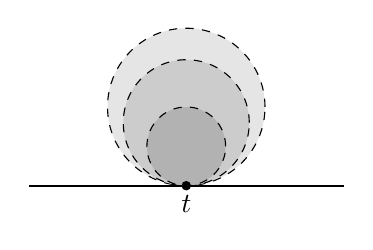
\begin{tikzpicture}
	\filldraw[dashed, fill=gray!20, opacity=40] (0, 1) circle[radius=1];
	\filldraw[dashed, fill=gray!40, opacity=40] (0, 0.8) circle[radius=0.8];
	\filldraw[dashed, fill=gray!60, opacity=40] (0, 0.5) circle[radius=0.5];
	\draw[fill=black] (0,0) circle[radius=1.5pt];
	\node at (0,0) [below] {$t$};
	\draw[thick] (-2,0) -- (2,0);
\end{tikzpicture}\end{center}
换言之, 对每个切 $\R^*$ 于 $t$ 的极限圆, 考虑它围出的圆盘 $H$ 并添入 $H^\circ \sqcup \{t\}$. 如果 $t=\infty$, 相应的子集化作 $\{\tau: \Im(\tau) > c \} \sqcup \{\infty\}$, 其中 $c \in \R_{>0}$; 圆盘模型上的图像兴许更清楚. 接着定义 $\mathcal{H}^*$ 的子集族 \index[sym1]{$H^\circ$}
\[ \mathscr{B} = \left\{ U: \mathcal{H}\; \text{中开集} \right\} \sqcup \left\{H^\circ \sqcup \{t \}: t \in \mathcal{C}_\Gamma, \; H\; \text{是切 $t$ 的极限圆盘} \right\}. \]
极易验证
\begin{inparaenum}[(1)]
	\item $\bigcup \mathcal{B} = \mathcal{H}^*$,
	\item 设 $U, U' \in \mathcal{B}$ 而 $x \in U \cap U'$, 则存在 $W \in \mathcal{B}$ 使得 $x \in W \subset U \cap U'$.
\end{inparaenum}
因此 $\mathcal{B}$ 作为一族基 (见 \cite[\S 2.6]{Xiong}) 确定了 $\mathcal{H}^*$ 上的拓扑; 易见
\begin{compactitem}
	\item $\mathcal{H}^*$ 满足第二可数公理 (有可数基), 见引理 \ref{prop:cusp-countable};
	\item $\mathcal{C}_\Gamma$ 是 $\mathcal{H}^*$ 的离散子集,
	\item 此拓扑在开子集 $\mathcal{H}$ 上诱导它原有的拓扑,
	\item $\Gamma$ 在 $\mathcal{H}^*$ 上连续地作用.
\end{compactitem}

兹考虑自然嵌入
\[ \Gamma \backslash \mathcal{H} \hookrightarrow \Gamma \backslash \mathcal{H}^*. \]
它对两边的商拓扑连续, 并且因为 $\mathcal{H} \hookrightarrow \mathcal{H}^*$ 为开, 它实际还是开嵌入. 现在着手赋予 $\Gamma \backslash \mathcal{H}^*$ 自然的 Riemann 面结构, 思路类似于 \S\ref{sec:Y-charts}, 但需要更多技术准备.

\begin{lemma}\label{prop:horocycle-immersion-aux}
	考虑 $\alpha \in \SL(2,\R)$ 和 $t := \alpha^{-1}\infty \in \R^*$. 定义 $H^\circ_c := \{\tau \in \mathcal{H}: \Im(\tau) > c \}$. 假设 $\infty, t \in \mathcal{C}_\Gamma$, 则对任意 $c > 0$, 存在 $c' > 0$ 使得
	\[ \forall \gamma \in \Gamma, \; \left[ (\gamma\alpha^{-1} H^\circ_c) \cap H^\circ_{c'} \neq \emptyset \implies \gamma t = \infty \right]. \]
\end{lemma}
\begin{proof}
	设若不然, 则存在点列 $\tau_n = x_n + iy_n$ 以及 $\gamma_n \in \Gamma$, 使得
	\[ y_n > c, \quad \Im\left(\gamma_n \alpha^{-1}\tau_n\right) \to +\infty, \quad \gamma_n t \neq \infty. \]
	置 $\eta_n := \gamma_n \alpha^{-1} = \twomatrix{a_n}{b_n}{c_n}{d_n}$, 因而 $\eta_n \infty \neq \infty$, 而且
	\[ \Im(\eta_n \tau_n) = \frac{y_n}{|c_n \tau_n + d_n|^2} = \frac{y_n}{(c_n x_n + d_n)^2 + (c_n y_n)^2} < c^{-1} |c_n|^{-2}. \]
	左式趋近 $\infty$, 所以 $c_n \to 0$. 又因为 $\infty, t \in \mathcal{C}_\Gamma$, 存在抛物元
	\[ \xi = \begin{pmatrix} 1 & r \\ & 1 \end{pmatrix} \in \overline{\Gamma}_\infty, \quad \xi' = \alpha^{-1} \begin{pmatrix} 1 & s \\ & 1 \end{pmatrix} \alpha \in \overline{\Gamma}_t \]
	满足 $r,s > 0$. 将 $\eta_n$ 代以 $\xi^h \eta_n (\alpha \xi' \alpha^{-1})^k \in \Gamma \alpha^{-1}$ 不影响 $c_n$. 适当取 $h, k$ (依赖于 $n$) 以确保存在由 $r, s$ 确定之常数 $B \geq 0$, 使得
	\[ \forall n, \quad |a_n - 1| < B|c_n|, \quad |d_n - 1| < B|c_n|. \]
	于是 $a_n, c_n, d_n$ 皆有界. 最后
	\[ |b_n c_n| = \left| (a_n - 1) (d_n - 1) + (a_n - 1) + (d_n - 1) \right| \leq B^2 c_n^2 + 2B|c_n| \]
	表明 $b_n$ 也有界. 由 $\Gamma \alpha^{-1}$ 离散推知 $\eta_n$ 的选法有限, 于是 $n$ 充分大时 $c_n = 0$, 这与 $\eta_n \infty \neq \infty$ 矛盾.
\end{proof}

以下是引理 \ref{prop:nbhd-elliptic} 的类比. 这里的困难在于 $\Gamma$ 在 $\mathcal{C}_\Gamma$ 上不再是正常作用.
\begin{lemma}\label{prop:horocycle-immersion}
	对任意 $t \in \mathcal{C}_\Gamma$, 存在切 $t$ 的极限圆盘 $H$ 使得 $H^\circ$ 不含椭圆点, 而且
	\[ U := H^\circ \sqcup \{t\}, \quad \Gamma_t \backslash U \to \Gamma \backslash \mathcal{H}^* \; \text{是开嵌入}. \]
\end{lemma}
\begin{proof}
	一如既往, 调整 $\Gamma$ 后可假设 $t = \infty$. 引理 \ref{prop:cusp-stabilizer} 表明 $\overline{\Gamma_t}$ 由某个 $\twomatrix{1}{x}{}{1}$ 生成, 其中 $x \neq 0$. 我们断言当 $a \gg 0$ 时, $H^\circ := \{\tau: \Im(\tau) > a \}$ 满足于: 对任意 $\tau, \tau' \in H^\circ$,
	\[ \forall \gamma \in \Gamma, \; \left[ \gamma\tau=\tau' \implies \gamma \in \Gamma_t \right]. \]
	诚然, 在引理 \ref{prop:horocycle-immersion-aux} 中取 $t=\infty$, $\alpha=1$ 和任意 $c>0$, 再取 $a := \max\{c,c'\}$ 便是.
	
	既然 $\R^* \cap U = \{t\}$, 由此可知 $\iota: \Gamma_t \backslash U \to \Gamma \backslash \mathcal{H}^*$ 为单射. 因为 $\twomatrix{1}{x}{}{1}$ 在 $\mathcal{H}$ 上无不动点, $\iota$ 单也蕴涵 $H^\circ$ 不含椭圆点.
	
	显然 $\iota$ 连续. 任意 $\Gamma_t \backslash U$ 中的开子集拉回为 $\mathcal{H}^*$ 的开子集, 再透过商映射映为 $\Gamma \backslash \mathcal{H}^*$ 的开子集 (引理 \ref{prop:quotient-common-sense}), 故 $\iota$ 为开嵌入. 明所欲证.
\end{proof}

至此已经可以确定 $\Gamma \backslash \mathcal{H}^*$ 的基本拓扑性质.
\begin{lemma}\label{prop:X-curve-topology}
	商空间 $\Gamma \backslash \mathcal{H}^*$ 是满足第二可数公理的连通 Hausdorff 空间.
\end{lemma}
\begin{proof}
	既然 $\mathcal{H}^*$ 满足第二可数公理, $\Gamma \backslash \mathcal{H}^*$ 亦然 (引理 \ref{prop:quotient-common-sense}). 以下证明 Hausdorff 性质.
	\begin{itemize}
		\item 分离 $\mathcal{H}$ 的点: 开子集 $\Gamma \backslash \mathcal{H}$ 由定义--定理 \ref{prop:Y-chart} 已知是 Hausdorff 的.
		\item 分离尖点与 $\mathcal{H}$ 的点: 照例化约到尖点来自 $\infty$ 的情形, 考虑 $\eta$ 在 $\mathcal{H}$ 中的紧邻域 $K$. 在引理 \ref{prop:horocycle-immersion-aux} 中代入 $\alpha = 1$ 和 $t = \infty$, 选取足够小的 $c$ 并且加大相应的 $c'$, 可以进一步要求引理中的 $c, c'$ 满足
		\[ \tau \in K \implies c < \Im(\tau) < c'; \]
		相应地定义 $H^\circ_c, H^\circ_{c'}$. 我们断言 $H^\circ_{c'} \sqcup \{\infty\}$ 和 $K$ 在 $X(\Gamma)$ 中的像无交.
		
		设若不然, 则存在 $\gamma \in \Gamma$ 使得 $\gamma H^\circ_c \cap H^\circ_{c'} \supset \gamma K \cap H^\circ_{c'} \neq \emptyset$. 引理 \ref{prop:horocycle-immersion-aux} 蕴涵 $\gamma \infty = \infty$, 从而根据引理 \ref{prop:cusp-stabilizer}, $\gamma K$ 是 $K$ 的一个横移, 它不可能有虚部 $> c'$ 的点. 矛盾.
		\item 分离尖点: 同样化约到两尖点来自 $t, \infty \in \mathcal{C}_\Gamma$ 情形, 再取 $\alpha \in \SL(2,\R)$ 使 $t = \alpha^{-1}\infty$. 以下沿用引理 \ref{prop:horocycle-immersion-aux} 的记号. 若 $t, \infty$ 在 $\Gamma \backslash \mathcal{H}^*$ 中的像无不交的邻域, 那么对任意 $c, c' > 0$, 总存在 $\gamma \in \Gamma$ 使得 $\gamma\alpha^{-1}(H^\circ_c) \cap H^\circ_{c'} \neq \emptyset$; 根据引理 \ref{prop:horocycle-immersion-aux}, 对固定之 $c$ 取 $c' \gg 0$ 必导致 $\gamma t = \infty$, 这就意谓 $t,\infty$ 属于同一个尖点.
	\end{itemize}
	最后, 连通性是 $\mathcal{H}^*$ 连通的直接结论.
\end{proof}

现在开始为 $\Gamma\backslash\mathcal{H}^*$ 在尖点附近构造坐标卡. 思路基于不变量, 同引理 \ref{prop:glueing-holomorphy} 平行.

\begin{lemma}\label{prop:glueing-holomorphy-cusp}
	对任意 $x \in \Gamma \backslash \mathcal{C}_\Gamma$, 存在开邻域 $V \ni x$ 和同胚 $z: V \rightiso \mathcal{D}$, 满足于下述条件.
	\begin{compactitem}
		\item 存在 $t \in \pi^{-1}(x)$ 及其开邻域 $U$ 使得
		\begin{compactitem}
			\item $U$  中无椭圆点;
			\item $U$ 对 $\Gamma_t$ 作用不变, $U \cap \mathcal{C}_\Gamma = \{t\}$, 而且有无交并分解
			\[ \pi^{-1}(V) = \bigsqcup_{\gamma \in  \Gamma/\Gamma_t} \gamma U \quad \text{(作为拓扑空间)}. \]
		\end{compactitem}
		不同的 $t \in \pi^{-1}(x)$ 之间被 $\Gamma$ 搬运, 故上述性质和 $x$ 实质无关.
		\item $z(x) = 0$;
		\item 对于任何非空开子集 $\mathcal{V} \subset V$ 和函数 $f^\flat: z(\mathcal{V}) \to \CC$, 命 $f := f^\flat \circ z \circ \pi: \pi^{-1}(\mathcal{V}) \to \CC$, 那么 $f^\flat$ 全纯当且仅当 $\pi^{-1}(\mathcal{V}) \subset \mathcal{H}^*$ 上的 $\Gamma$-不变函数 $f$ 满足
		\begin{compactitem}
			\item $f$ 在 $\pi^{-1}(\mathcal{V} \smallsetminus \{x\})$ 上全纯, 而且
			\item $f$ 可以连续地延拓到 $\pi^{-1}(\mathcal{V})$.
		\end{compactitem}
	\end{compactitem}
	这样的开邻域 $V \ni x$ 可以取得任意小.
\end{lemma}
\begin{proof}
	对任意 $t \in \mathcal{C}_\Gamma$ 选取如引理 \ref{prop:horocycle-immersion} 的 $H^\circ$ 和开子集
	\[\begin{tikzcd}[row sep=tiny]
		& \mathcal{H}^* \arrow[twoheadrightarrow, r, "\pi"] & \Gamma \backslash \mathcal{H}^* & \\
		U \arrow[phantom, r, ":=" description] & H^\circ \sqcup \{t\} \arrow[twoheadrightarrow, r] \arrow[phantom, u, "\subset" description, sloped] & \pi(U) \arrow[phantom, r, "=:" description] \arrow[phantom, u, "\subset" description, sloped] & V
	\end{tikzcd}\]
	关于 $U$ 的条件自动满足. 接着构造局部坐标 $z$. 存在 $\alpha \in \SL(2,\R)$ 映 $t$ 为 $\infty$. 对于选定之 $\alpha$, 根据引理 \ref{prop:cusp-stabilizer}
	\begin{equation}\label{eqn:cusp-width}
		\PSL(2,\R) \supset \overline{\alpha\Gamma_t \alpha^{-1}} = \lrangle{\twomatrix{1}{h}{}{1}},
	\end{equation}
	其中 $h \in \R_{>0}$ 由 $t$, $\alpha$ 和 $\overline{\Gamma}$ 唯一确定. 定义
	\[\begin{tikzcd}[row sep=tiny]
		\Gamma_t \backslash U \arrow[r, "z"] & \CC \\
		\Gamma_t \cdot \tau \arrow[mapsto, r] \arrow[phantom, u, "\in" description, sloped] & \exp\left(2\pi i \cdot \frac{\alpha(\tau)}{h} \right). \arrow[phantom, u, "\in" description, sloped]
	\end{tikzcd}\]
	一般而言, $\alpha$ 的选取可以差一个形如 $\twomatrix{a}{b}{}{a^{-1}}$ 的左乘, 相应地 \eqref{eqn:cusp-width} 中的 $h \leadsto a^2 h$, 故坐标按
	\begin{align*}
		z(\Gamma_t \cdot \tau) & = \exp\left(2\pi i \cdot \frac{\alpha(\tau)}{h} \right) \\
		& \leadsto \exp\left( 2\pi i \cdot \frac{a^2 \alpha(\tau) + ab}{a^2 h} \right) = z(\Gamma_t \cdot \tau) \exp\left( \frac{2\pi i b}{ah} \right)
	\end{align*}
	变化. 如果 $t = \infty$, $\alpha=1$ 而 $H^\circ = \{ \tau: \Im(\tau) > c\}$, 那么 $z$ 显然给出同胚 $V \rightiso \left\{z \in \CC: |z| < e^{-2\pi c/h} \right\}$, 满足 $z^{-1}(0) = \{t\}$. 透过 $\alpha$ 的搬运, 一般情形准此可知.
	
	最后验证全纯函数的刻画. 化约到 $t=\infty$ 情形. 一如引理 \ref{prop:glueing-holomorphy}, 一切归结为以下事实: 设 $\mathcal{W} \subset \{\tau: \Im(\tau) > c \}$ 是对平移 $\tau \mapsto \tau + h$ 不变的开集, 定义 $\mathcal{D}$ 中开集 $\mathcal{W}^\flat := \exp(2\pi i/h \cdot \mathcal{W})$, 那么一个函数 $g^\flat: \mathcal{W}^\flat \to \CC$ 全纯当且仅当 $g(\tau) := g^\flat(\exp(2\pi i\tau /h))$ 满足
	\begin{compactitem}
		\item $g$ 在 $\mathcal{W}$ 上全纯;
		\item 若 $\mathcal{W}$ 中元素的虚部无上界, 那么 
		\[ \lim_{\substack{\tau \in \mathcal{W} \\ \Im(\tau) \to +\infty}} g(\tau) \quad \text{存在}. \]
	\end{compactitem}
	一如既往, 问题的根本在 $\infty$ 附近, 所需论证是初等的.
\end{proof}

综之得到 $\Gamma \backslash \mathcal{C}_\Gamma$ 在 $\Gamma \backslash \mathcal{H}^*$ 中的一族开复盖, 其中每个开集 $V = \pi(U)$ 都带有坐标函数 $z$, 而且 $\Gamma$-不变函数 $f := z \circ \pi: \pi^{-1}V \to \CC$ 具有引理断言的性质.

\begin{definition-theorem} \index[sym1]{$X(\Gamma)$}
	相对于定义--定理 \ref{prop:Y-chart} 和引理 \ref{prop:glueing-holomorphy-cusp} 给出的坐标卡, $\Gamma \backslash \mathcal{H}^*$ 是连通 Riemann 曲面, 记为 $X(\Gamma)$, 它包含 $Y(\Gamma)$ 作为稠密开子集. 我们也称 $X(\Gamma)$ 为 $\Gamma$ 对应的\emph{模曲线}.
\end{definition-theorem}
\begin{proof}
	引理 \ref{prop:X-curve-topology} 已确立连通复流形所需的基本拓扑条件. 剩下的任务是证明尖点附近的任两个坐标卡皆相容. 此处论证和定义--定理 \ref{prop:Y-chart} 类似, 唯一差别在于必须兼用引理 \ref{prop:glueing-holomorphy} 和 \ref{prop:glueing-holomorphy-cusp} 以刻画尖点附近的复结构.
\end{proof}

\begin{remark}
	从复结构的观点看, 引理 \ref{prop:glueing-holomorphy-cusp} 构造的局部坐标 $z$ 表明 $X(\Gamma)$ 在尖点附近都同构于 $\mathcal{D}$. 但从 Riemann 度量的立场, 尖点附近的几何图像则如
	\begin{center}\begin{tikzpicture}[scale=1.2]
		\coordinate (A) at (0, 0);
		\coordinate (B) at (3, 0);
		\begin{scope}[shift=(A)]
			\draw (-0.5, 0) -- (-0.5, 2) coordinate[midway] (X);
			\draw (0.5, 0) -- (0.5, 2) coordinate[midway] (Y);
			\draw[thick, <->] (X) -- (Y) node[midway, below] {$h$};
		\end{scope}
		\draw[-Latex, line width=3pt] (1.2, 1.2) -- (2.3, 1.2) node[midway, above, inner sep=0.8em] {\footnotesize 取商};
		\begin{scope}[shift=(B)]
			\draw (-0.8, 0) .. controls (-0.5,  0.2) and (-0.2, 0.5) .. (-0.1, 2) coordinate[midway] (X);
			\draw (0.8, 0) .. controls (0.5,  0.2) and (0.2, 0.5) .. (0.1, 2) coordinate[midway] (Y);
			\draw[thick] (X) to[bend right] (Y);
			\draw[thick, dashed] (Y) to[bend right] (X);
			\draw[-Latex] (1.8, 0.5) -- (1.8, 1.5) node[above] {\footnotesize 趋向尖点}; 
		\end{scope}
	\end{tikzpicture}\end{center}
	此处假定尖点来自上半平面的 $\infty$, 而 $h$ 如 \eqref{eqn:cusp-width}. 随着极限圆收拢到 $\infty$, 它在 $Y(\Gamma)$ 中的像长度趋近于 $0$. 和注记 \ref{rem:Y-metric} 类似, 尖点处同样是度量的奇点.
\end{remark}

\begin{exercise}
	证明 $Y(\Gamma)$ 紧蕴涵 $\Gamma$ 无尖点.
\end{exercise}

\begin{exercise}
	参照定义 \ref{def:branched-covering}, 验证商映射 $\mathcal{H}^* \to X(\Gamma)$ 是分歧复叠, 其中分歧指数无穷的部分正好是 $\mathcal{H}^* \smallsetminus \mathcal{H} = \mathcal{C}_\Gamma$; 试描述其它点的样貌和分歧指数.
\end{exercise}

\section{同余子群情形}\label{sec:cong-compactification}
设 $\Gamma, \Delta$ 为 $\SL(2,\R)$ 的离散子群, $\Delta \subset \Gamma$, 那么 $\mathcal{C}_\Delta \subset \mathcal{C}_\Gamma$, 相应地得到连续满射 $f: X(\Delta) \to X(\Gamma)$. 请先回忆分歧复叠的定义 (参阅 \S\ref{sec:branched-covering}).

\begin{proposition}\label{prop:commensurable-covering}
	设 $(\Gamma:\Delta)$ 有限, 则 $f: X(\Delta) \to X(\Gamma)$ 是有限分歧复叠, $\deg(f) = \left( \overline{\Gamma} : \overline{\Delta} \right)$. 记 $\xi \in \mathcal{H} \sqcup \mathcal{C}_\Delta$ 在 $X(\Delta)$ 中的像为 $x$, 那么 $f$ 在 $x$ 处的分歧指数为 $e(x) = \left( \overline{\Gamma}_\xi : \overline{\Delta}_\xi \right)$.
\end{proposition}

\begin{proof}
	在椭圆点和尖点 (可数个) 之外, 映射 $f$ 是 $\left( \overline{\Gamma} : \overline{\Delta} \right)$ 对 $1$ 的, 其余点处的纤维可能变小. 以下验证分歧复叠的性质.

	考虑 $y \in Y(\Gamma)$ 及代表元 $\eta \in \mathcal{H}$. 对之使用 \S\ref{sec:Y-charts} 构造的开邻域 $V \simeq \Gamma_\eta \backslash U$ (设 $U \ni \eta$), 回忆到在圆盘模型下 $U$ 对应到半径 $\epsilon < 1$ 的开圆盘 $U'$. 回顾 \S\ref{sec:Y-charts} 的构造, 取 $\epsilon \ll 1$ 可确保 $U$ 对 $\Gamma_\eta$ 和 $\Delta_\eta$ 的商同时给出 $Y(\Gamma)$ 和 $Y(\Delta)$ 在 $\eta$ 处的坐标卡, 而 $f^{-1}(V)$ 可以写成如下形式的有限无交并
	\[ f^{-1}(V) = V_1 \sqcup \cdots \sqcup V_r, \quad V_i = \Delta_{\gamma_i \eta} \big\backslash \gamma_i U, \quad \gamma_i \in \Gamma. \]
	因此, 对每个 $1 \leq i \leq r$ 皆有交换图表
	\[\begin{tikzcd}
		V_i \arrow[d, "\simeq"', "{\gamma_i^{-1}}"] \arrow[r, "f"] & V \\
		\Delta_\eta \backslash U \arrow[d, "\simeq"', "D^{-1}"] \arrow[r, "\text{商}"] & \Gamma_\eta \backslash U \arrow[d, "\simeq", "D^{-1}"'] \arrow[u, "\simeq"'] \\
		\mu_h \backslash U' \arrow[r, "\text{商}"] \arrow[d, "{w \mapsto \epsilon^{-h} w^h}"', "\simeq"] & \mu_k \backslash U' \arrow[d, "{w \mapsto \epsilon^{-k} w^k}", "\simeq"'] \\
		\mathcal{D} \arrow[r, "{z \mapsto z^e}"'] & \mathcal{D}
	\end{tikzcd} \quad
	\begin{array}{rl}
		h & := \left| \overline{\Delta_\eta} \right| , \\
		k & := \left| \overline{\Gamma_\eta} \right| , \\
		e & := \frac{k}{h} = \left(\overline{\Gamma_\eta} : \overline{\Delta_\eta}\right),
	\end{array}\]
	这就在 $y$ 附近验证了分歧复叠和分歧指数的性质. 尖点附近可依样画葫芦, 细节留给读者.
\end{proof}

\begin{corollary}
	若 $\SL(2, \R)$ 的离散子群 $\Gamma$ 和 $\Delta$ 可公度, 则 $X(\Gamma)$ 紧当且仅当 $X(\Delta)$ 紧.
\end{corollary}
\begin{proof}
	问题化到 $\Delta \subset \Gamma$ 的情形. 代入命题 \ref{prop:commensurable-covering} 并运用命题 \ref{prop:branched-compactness} 即可.
\end{proof}

现在可对 $X(\Gamma)$ 在同余子群情形的紧性给出直接证明.
\begin{proposition}
	若 $\SL(2, \R)$ 的离散子群 $\Gamma$ 与 $\SL(2, \Z)$ 可公度, 则 $X(\Gamma)$ 紧; 作为特例, 同余子群给出的 $X(\Gamma)$ 皆紧. 进一步, $X(\SL(2,\Z))$ 同胚于球面 $\mathbb{S}^2$.
\end{proposition}
\begin{proof}
	第一部分的断言简化到 $\Gamma = \SL(2,\Z)$ 的情形. 以下论证依赖 \eqref{eqn:fundamental-domain-full} 给出的基本区域 $\mathcal{F} = \left\{\tau: |\Re(\tau)| \leq \frac{1}{2}, \; |\tau| \geq 1 \right\}$.
	
	考虑 $S = \twomatrix{}{-1}{1}{}$ 和 $T = \twomatrix{1}{1}{}{1}$ 分别在 $\mathcal{F}$ 的底部和两边的作用, 我们知道将 $\partial\mathcal{F} \sqcup \{\infty\}$ 如下粘合, 得到的空间同胚于 $X(\SL(2,\Z))$ (参照引理 \ref{prop:full-fundamental-domain-aux}):
	\begin{center}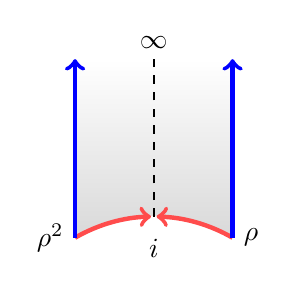
\begin{tikzpicture}[scale=2]
		\fill[draw=white, shading=axis, bottom color=gray!30, top color=white, opacity=40] (-0.5, 2) -- (120:1) arc(120:60:1) -- (0.5, 2) --cycle;
		\draw[ultra thick, color=red!70, ->] (120:1) node[left, color=black] {$\rho^2$} arc(120:91:1);
		\draw[ultra thick, color=red!70, ->] (60:1) node[right, color=black] {$\rho$} arc (60:89:1);
		\draw[ultra thick, color=blue, ->] (120:1) -- (-0.5, 2);
		\draw[ultra thick, color=blue, ->] (60:1) -- (0.5, 2);
		\node at (0, 0.8) {$i$};
		\draw[thick, dashed] (0,1) -- (0,2) node[above] {$\infty$};
		\end{tikzpicture}\end{center}
	这里要求对粘合相同颜色的边界, 箭头所示的方向必须符合. 如将一切放到圆盘模型上, 明白可见这是一个三角剖分, 相当于粘合
	\begin{center}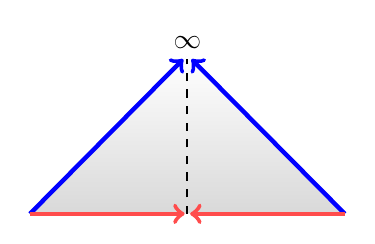
\begin{tikzpicture}
		\coordinate (A) at (0,2);
		\coordinate (B) at (-2,0);
		\coordinate (C) at (2,0);
		\coordinate (M) at (0,0);
		\fill[draw=white, shading=axis, bottom color=gray!30, top color=white, opacity=40] (A) -- (B) -- (C) --cycle;
		\draw[ultra thick, color=blue, ->] (B) -- ([xshift=-1.5pt, yshift=-1pt]A);
		\draw[ultra thick, color=blue, ->] (C) -- ([xshift=1.5pt, yshift=-1pt]A);
		\draw[ultra thick, color=red!70, ->] (B) -- ([xshift=-1pt]M);
		\draw[ultra thick, color=red!70, ->] (C) -- ([xshift=1pt]M);
		\draw[thick, dashed] (M) -- ([yshift=-1pt]A) node[above] {$\infty$};
	\end{tikzpicture}\end{center}
	上图既是紧拓扑空间, 粘合得到的商空间自然也是紧的. 这也相当于将 $X(\SL(2,\Z))$ 实现为一个单纯复形, 其中有两个 $2$ 维单纯形, 见 \S\ref{sec:Riemann-Hurwitz} 的讨论.

	读者可以尝试去直观粘合的产物同胚于 $\mathbb{S}^2$, 或者是计算复形的点, 线, 面个数, 用 Euler 示性数和闭曲面的分类理论来论证.
\end{proof}

\begin{convention} \index[sym1]{$X(N), X_1(N), X_0(N)$} \index[sym1]{$Y(N), Y_1(N), Y_0(N)$}
	习见的符号是 $X(N) := X(\Gamma(N))$, $X_1(N) := X(\Gamma_1(N))$, $X_0(N) := X(\Gamma_0(N))$; 特别地, $X(1) = X(\SL(2,\Z))$. 类似地, $Y(N) := Y(\Gamma(N))$, $Y_1(N) := Y(\Gamma_1(N))$, $Y_0(N) := Y(\Gamma_0(N))$.
\end{convention}

已知亏格为 $0$ 的紧 Riemann 曲面必同构于 Riemann 球面 $\CC \sqcup \{\infty\}$, 或者说是复射影直线 $\PP^1$, 于是上述论证实际确定了 Riemann 曲面 $X(1)$. 事实上有更精确的描述如下.

\begin{theorem}\label{prop:j-Hauptmodul}
	定义 \ref{def:modular-invariant} 引进的模不变量 $j(\tau) = E_4(\tau)^3/\Delta(\tau)$ 给出紧 Riemann 曲面之间的同构 $j: X(1) \rightiso \PP^1$.
\end{theorem}
\begin{proof}
	在 \S\ref{sec:j-invariant} 已经说明 $j$ 对 $\SL(2,\Z)$ 作用不变, 并给出紧 Riemann 曲面
	\[ X(1) = \SL(2,\Z) \backslash \mathcal{H} \sqcup \{\infty\} \]
	上的亚纯函数: 它在 $\mathcal{H}$ 上无极点, 在 $\infty$ 处则有一阶极点 (事实上 $j(\tau) = q^{-1} + 744 + \cdots$), 因此 $j$ 的极点计重数恰有 $1$ 个. 由此立见态射 $j: X(1) \to \PP^1$ 满足 $\deg(j) = 1$ (推论 \ref{prop:value-degree}), 因而是紧 Riemann 曲面的同构 (命题 \ref{prop:degree-1}).
\end{proof}

凡是亏格 $0$ 的模曲线 (例如当 $1 \leq N \leq 10$ 或 $N=12$ 时的 $X_1(N)$) 都带有类似的模函数, 习惯称为主模函数\footnote{德文: \textit{Hauptmodul}}.

\begin{example} \index{Picard 小定理}
	在尖点 $\infty$ 和椭圆点 $i, \rho := \frac{1 + \sqrt{-3}}{2}$ 处, $j$ 的取值可以确定为
	\begin{equation}\label{eqn:j-value}
		j(\infty)=\infty, \quad j(i)=1728, \quad j(\rho) = 0;
	\end{equation}
	尖点 $\infty$ 处的取值已在 \S\ref{sec:j-invariant} 求出, 而后两个值的计算尚需周折, 将在例 \ref{eg:j-computation} 予以说明. 姑且承认 \eqref{eqn:j-value}, 复变函数论中著名的 \emph{Picard 小定理}便有一个简单证明. 该定理断言: 任意非常值全纯函数 $f: \CC \to \CC$ 的取值至多略过一个点.
	
	假设 $f$ 略过至少两个值 $v,w$, 取 $\gamma \in \PGL(2,\CC)$ 映 $(v,w,\infty)$ 为 $(0,1728,\infty)$, 这般 $\gamma$ 可以用交比 \eqref{eqn:cross-ratio-transitivity} 描述, 因此不妨设 $0, 1728 \notin f(\CC)$. 命 $X(1)' \subset X(1)$ 为 $\{\rho ,i, \infty\}$ 的 $\Gamma(1)$-轨道的补集, 那么 $j(X(1)') = \PP^1 \smallsetminus \{0,1728,\infty\}$; 再命 $\mathcal{H}' \subset \mathcal{H}$ 为 $i, \rho$ 的 $\Gamma(1)$-轨道的补集. 考虑 Riemann 曲面范畴中的交换图表 (先看实线部分):
	\[\begin{tikzcd}
		\mathcal{H}' \arrow[twoheadrightarrow, r] & X(1)' \arrow[d, "j", "\simeq"'] \\
		\CC \arrow[dashed, u, "\exists g"] \arrow[r, "f"] & \PP^1 \smallsetminus \{0,1728,\infty\}
	\end{tikzcd}\]
	由于扣除了尖点和椭圆点, $\mathcal{H}' \twoheadrightarrow X(1)'$ 是复叠映射: 它实际还是连通的 $\PSL(2,\Z)$-主丛. 既然 $\CC$ 单连通, 复叠映射理论遂给出使上图交换之 $g$ (可参阅 \cite[定理 5.3]{You}); 而 $g$ 也是全纯的. 最后考虑 $z \mapsto \exp(2\pi i g(z))$, 它是从 $\CC$ 到单位圆盘的全纯映射, 根据 Liouville 定理必为常值. 相应地 $g$ 和 $f$ 必为常值. 明所欲证.
\end{example}

\section{Siegel 定理与紧化}\label{sec:Siegel-thm}
令 $\Gamma$ 为 $\SL(2,\R)$ 的离散子群,按注记 \ref{rem:Y-metric} 用基本区域的面积定义 $\mes(Y(\Gamma))$. 上节已向 $Y(\Gamma)$ 添入尖点, 得到 Riemann 曲面 $X(\Gamma)$, 然而需要进一步的条件来保证 $X(\Gamma)$ 紧, 这主要是 Siegel 定理 \ref{prop:Fuchsian-1st-kind} 的内容.

以下需要 \S\ref{sec:Dirichlet-domain} 的 Dirichlet 区域理论, 包括其中的边和尖点等概念, 见定义 \ref{def:sides}. 回忆到边和 Dirichlet 区域边界上的极大测地线段不是同一个概念.

取定非椭圆点 $x_0$. 对 Dirichlet 区域 $D(x_0)$ 加进其无穷远点, 得到 $D(x_0)^*$. 着手证明关键的 Siegel 定理前, 有必要加深对这些无穷远点及其稳定化子群的了解.
\begin{lemma}\label{prop:parabolic-stabilizer-aux}
	假定 $\xi$ 是 $D(x_0)^*$ 的尖点, 那么 $\overline{\Gamma}_\xi$ 的非平凡元皆是抛物元.
\end{lemma}
\begin{proof}
	使用反证法. 非抛物元 $\gamma \in \overline{\Gamma}_\xi \smallsetminus \{1\}$ 必是双曲元, 它恰有两个不动点 $\xi, \eta$, 都落在边界上. 存在唯一的测地线 $\mathcal{A}$ 从 $\eta$ 流向 $\xi$; 另一方面, 存在从某点 $x \in D(x_0)$ 流向 $\xi$ 的测地射线 $\mathcal{B}$, 与 $\mathcal{A}$ 平行, 并且全程落在 $D(x_0)$ 内. 如果在上半平面里取 $\xi = \infty$, 图像将是直观的:
	\begin{center}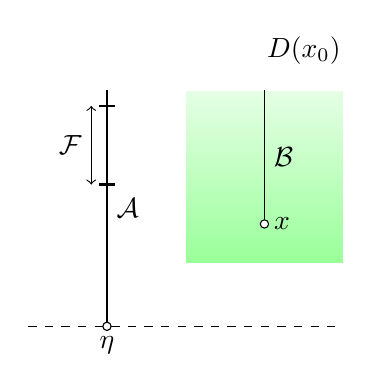
\begin{tikzpicture}
		\fill[draw=white, shading=axis, bottom color=green!40, top color=green!10] (1, 3) -- (1, 0.8) -- (3, 0.8) -- (3, 3) --cycle;
		\draw (0, 0) -- (0, 3) node[midway, right] {$\mathcal{A}$};
		\draw (2, 1.3) -- (2, 3) node[midway, right] {$\mathcal{B}$};
		\draw[thick] (-0.1, 1.8) -- (0.1, 1.8);
		\draw[thick] (-0.1, 2.8) -- (0.1, 2.8);
		\draw[<->] (-0.2, 1.8) -- (-0.2, 2.8) node[midway, left] {$\mathcal{F}$};
		\draw[dashed] (-1, 0) -- (3, 0);
		\draw[fill=white] (0,0) circle[radius=1.5pt] node[below] {$\eta$};
		\node at (2.5, 3.5) {$D(x_0)$};
		\draw[fill=white] (2, 1.3) circle[radius=1.5pt] node[right] {$x$};
	\end{tikzpicture}\end{center}

	于是 $\gamma$ 诱导 $\mathcal{A}$ 到自身的保向等距映射. 相对于 $\mathcal{A}$ 的测地坐标, $\gamma|_{\mathcal{A}}$ 无非是平移. 故存在 $\mathcal{A}$ 中一个有限长度的线段 $\mathcal{F}$, 使得 $\mathcal{F}$ 是 $\gamma|_{\mathcal{A}}$ 生成的群作用下的基本区域: 取 $\mathcal{F}$ 的长度为 $\gamma|_{\mathcal{A}}$ 的平移步长便是. 在 $D(x_0) \cap \mathcal{B}$ 中取点列 $b_1, b_2, \ldots$ 趋向 $\xi$, 并在 $\mathcal{A}$ 中取 $a_1, a_2, \ldots \to \xi$ 使得 $n \to \infty$ 时 $d(a_n, b_n) \to 0$: 对于上图的情景, 取 $a_n \in \mathcal{A}$ 使得 $\Im(a_n) = \Im(b_n)$ 便是.
	
	对所有 $n \geq 1$, 取 $k_n \in \Z$ 使得 $a_n \in \gamma^{k_n} \mathcal{F}$; 因为 $a_n$ 趋近边界, 必有 $|k_n| \to \infty$. 从 $d(a_n, b_n) = d\left( \gamma^{-k_n} a_n, \gamma^{-k_n} b_n \right) \to 0$ 推得 $d\left(\mathcal{F}, \gamma^{-k_n} b_n \right) \to 0$. 但 $\gamma^{-k_n} b_n \in \gamma^{-k_n} D(x_0)$, 于是当 $n \to +\infty$ 时紧集 $\mathcal{F}$ 附近簇拥了无穷多个 $D(x_0)$ 的相异 $\overline{\Gamma}$-平移像, 与基本区域 $D(x_0)$ 的局部有限性矛盾.
\end{proof}

\begin{proposition}\label{prop:parabolic-stabilizer}
	设 $\partial D(x_0)^*$ 由有限多个极大测地线段组成, 所有无穷远顶点都是尖点, 那么
	\begin{compactenum}[(i)]
		\item $D(x_0)^*$ 的边数和顶点数皆有限;
		\item 对所有无穷远顶点 $\xi$ 皆有 $\overline{\Gamma}_\xi \simeq \Z$, 由抛物元生成;
		\item $D(x_0)$ 仅包含有限多个 $\overline{\Gamma}$ 的椭圆点, 全落在 $\partial D(x_0)$ 上.
	\end{compactenum}
\end{proposition}
\begin{proof}
	先处理 (i). 须说明 $\partial D(x_0)$ 中每条极大测地线段仅由有限个边组成. 问题显然只可能发生在延伸到无穷远点的线段.
	
	取定 $\partial D(x_0)$ 中一条包含无穷多条边的极大测地线段, 不妨在上半平面中假设它形如 $[m, \infty]$, 其中 $m \in i\R_{\geq 0}$; 故 $\infty$ 是 $D(x_0)^*$ 的尖点. 包含于 $[m, \infty]$ 的边分作三类.
	\begin{compactdesc}
		\item[第一类] 形如 $[b, \infty]$ 的边, 这样的边至多仅一条.
		\item[第二类] 形如 $[m, a]$ 的边, 这样的边至多也仅一条.
		\item[第三类] 不属以上两类的边 $S \subset [m, \infty]$. 此时 $S$ 长度有限, 表成 $S = [m, \infty] \cap \gamma D(x_0)$ 的形式, 其中 $\gamma \in \overline{\Gamma} \smallsetminus \{1\}$, 如下图:
		\begin{center}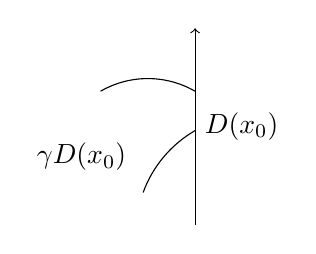
\begin{tikzpicture}[baseline=(X)]
			\draw[->] (0, -0.5) -- (0, 2) node[midway, right] {$D(x_0)$};
			\draw (0, 1.2) arc(60:120:1.2);
			\draw (0, 0.7) arc(120:160:1.5) node[midway, left=1em] {$\gamma D(x_0)$};
			\coordinate (X) at (0, 0.7);
		\end{tikzpicture}\end{center}
		上图的夹角都严格落在 $0$ 到 $\pi$ 之间, 所以 $S$ 包含于 $\partial(\gamma D(x_0))$ 的一条有限长度极大测地线段, 记为 $\tilde{S}$. 按边配对 (定义--命题 \ref{prop:side-pairing}) 将它搬回 $D(x_0)$ 的边 $T := \gamma^{-1} S$, 则 $T$ 也包含于 $\partial D(x_0)$ 的有限长度极大测地线段 $\gamma^{-1} \tilde{S}$.
	\end{compactdesc}

	只须说明第三类边的个数有限. 命 $\mathcal{T}$ 为所有包含于有限长度极大测地线段的边构成之集合; 证明之初的观察表明 $\mathcal{T}$ 有限. 令 $S = [m, \infty] \cap \gamma D(x_0)$ 和 $T = \gamma^{-1} S$ 如上, 则 $T \in \mathcal{T}$. 以下说明当 $S$ 遍历 $[m, \infty]$ 中的第三类边, 每个 $T \in \mathcal{T}$ 至多出现两次. 如此即说明 $[m, \infty]$ 所含边数有限.

	设边 $T \in \mathcal{T}$ 出现三次, 那么存在相异的 $\gamma_i \in \overline{\Gamma} \smallsetminus \{1\}$, $S_i \subset [m, \infty]$ 使得 $\gamma_i^{-1} S_i = T$, 其中 $i = 0, 1, 2$. 命 $\delta_i := \gamma_i \gamma_0^{-1}$, 那么 $\delta_i S_0 = S_i$. 因为 $S_0, S_1, S_2$ 都是 $[m, \infty]$ 的子线段, 长度非零, 故 $\delta_1, \delta_2 \in \overline{\Gamma} \smallsetminus \{1\}$ 皆映测地线 $[0, \infty]$ 为自身. 考虑 $\delta_1|_{[0, \infty]}$ 和 $\delta_2|_{[0, \infty]}$: 这两者相异, 其中或者有一个是非平凡的平移, 或者两者是相异反射, 那么 $\delta_1 \delta_2|_{[0, \infty]}$ 是非平凡的平移. 无论如何, 总能取到 $\delta \in \overline{\Gamma}$ 使 $\delta|_{[0, \infty]}$ 是非平凡的平移, 如是则 $\delta$ 给出 $\overline{\Gamma}_\infty$ 的双曲元 (参看例 \ref{eg:sliding}), 与引理 \ref{prop:parabolic-stabilizer-aux} 不符. 于是我们证明了 $D(x_0)^*$ 的边数有限, 从而顶点数亦有限.
	
	接着处理 (ii). 我们断言若无穷远顶点 $\xi$ 是尖的, 则 $\overline{\Gamma}_\xi$ 非平凡时必 $\simeq \Z$. 同样化到 $\xi = \infty$ 情形. 已知 $\overline{\Gamma}_\xi \smallsetminus \{1\}$ 由抛物元构成, 而 $\SL(2,\R)$ 中抛物元的特征值为 $\pm 1$, 故 $\overline{\Gamma}_\xi$ 是 $\twomatrix{1}{*}{}{1} \simeq \R$ 的离散子群. 应用命题 \ref{prop:disc-subgroup-circle} 立见 $\overline{\Gamma}_\xi \simeq \Z$.
	
	性质 (ii) 遂归结为对所有 $\xi$ 证明 $\overline{\Gamma}_\xi \neq \{1\}$. 设 $\eta, \eta'$ 为 $D(x_0)$ 之无穷远点, 若存在 $\gamma \in \overline{\Gamma}$ 使得 $\gamma\eta = \eta'$, 则记为 $\eta \sim \eta'$, 这给出等价关系. 一如 \eqref{eqn:delta-xi}, 我们有双射
	\begin{align*}
		\overline{\Gamma}_\xi \bigg\backslash \left\{ \delta \in \overline{\Gamma} : \delta D(x_0) \;\text{包含 $\xi$ 作为无穷远点} \right\} & \xrightarrow{1:1} \left\{\eta: \eta \sim \xi \right\} \\
		\overline{\Gamma}_\xi \delta & \longmapsto \delta^{-1}\xi .
	\end{align*}
	考虑所有这样的 $\delta D(x_0)$, 图示如下:
	\begin{center}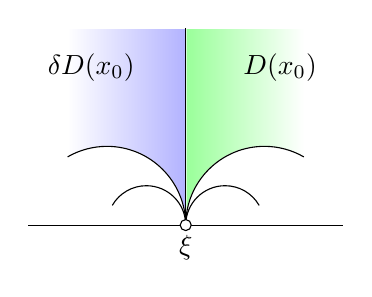
\begin{tikzpicture}
		\fill[draw=white, shading=axis, right color=white, left color=green!40] (0, 2.5) -- (0, 0) arc (180:60:1) -- (1.5, 2.5) --cycle;
		\fill[draw=white, shading=axis, left color=white, right color=blue!30] (0, 2.5) -- (0, 0) arc (0:120:1) -- (-1.5, 2.5) -- cycle;
		\draw (-2, 0) -- (2, 0);
%		\draw[dashed] (0, 1) circle[radius=1];
		\draw (0,0) arc (0:120:1);
		\draw (0,0) arc (180:60:1);
		\draw (0,0) arc (180:30:0.5);
		\draw (0,0) arc (0:150:0.5);
		\draw (0,0) -- (0, 2.5);
		\filldraw[fill=white] (0,0) circle[radius=0.07] node[below] {$\xi$};
		\node at (1.2, 2) {$D(x_0)$};
		\node at (-1.2, 2) {$\delta D(x_0)$};
	\end{tikzpicture}\end{center}
	假若 $\overline{\Gamma}_\xi = \{1\}$, 则因为无穷远顶点个数有限, 仅有限多个 $\delta D(x_0)$ 含 $\xi$ 为无穷远点, 此无可能: 取最左端之 $\delta D(x_0)$, 那么 $\delta D(x_0)^* = D(\delta x_0)^*$ 必有一边 $S$ 以 $\xi$ 为无穷远端点, 并落在 $\delta D(x_0)$ 左侧, 那么边配对将给出更靠左的一片 $\delta' D(x_0)$, 矛盾.

	最后处理 (iii). 按基本区域的性质, 椭圆点必落在 $\partial D(x_0)$ 上. 注记 \ref{rem:side-pairing} 表明这些点都是 $D(x_0)$ 细分后的顶点, 而从 (i) 已知顶点数量有限.
\end{proof}

现在可以进入正题.

\begin{definition}\index{Fuchs-qun!余有限 (cofinite)} \index{Fuchs-qun!第一类 (of the first kind)}
	若 $\SL(2, \R)$ 的离散子群 $\Gamma$ 满足 $\mathrm{vol}(Y(\Gamma)) < +\infty$, 则称为\emph{余有限 Fuchs 群}. \footnote{在 \cite{Mi89} 中称为第一类 Fuchs 群.}
\end{definition}

\begin{theorem}[C.\ L.\ Siegel, 见 {\cite[Theorem 1.9.1]{Mi89}}, {\cite[Theorem 13.1]{Kat10}}]\label{prop:Fuchsian-1st-kind}
\index{cediduobianxing}
	对 $\SL(2,\R)$ 的离散子群 $\Gamma$, 以下陈述等价:
	\begin{compactenum}[(i)]
		\item 若 $x_0$ 非椭圆点, 则 Dirichlet 区域 $D(x_0)$ 的边数有限, 所有无穷远处的顶点皆尖.
		\item $\Gamma$ 是余有限 Fuchs 群.
	\end{compactenum}
	当上述条件成立时, $D(x_0)$ 中的椭圆点个数有限, 全落在 $\partial D(x_0)$ 上, 而且对于 $D(x_0)$ 在无穷远处的每个顶点 $\xi$, 稳定化子群 $\overline{\Gamma}_\xi \simeq \Z$ 由抛物元生成.
\end{theorem}
\begin{proof}
	若存在非椭圆点 $x_0$ 使 $D(x_0)$ 具有断言的性质, 则定理 \ref{prop:Gauss-Bonnet} 说明其测度有限. 以下证明另一方向, 设 $x_0$ 非椭圆点, $D(x_0)$ 面积有限. 采取 \S\ref{sec:disc-model} 的圆盘模型 $\mathcal{D}$, 故无穷远点都落在边界 $|z| = 1$ 上.
	
	首先证明 $D(x_0)$ 的无穷远点个数有限. 任选其中有限多个 $x_1, \ldots, x_N$ (无妨设 $N \geq 3$), 以测地线按逆时针顺序相连, 得到 $\mathcal{D}$ 中一个测地多边形 $P$, 而且 $D(x_0)$ 的测地凸性蕴涵 $P \subset D(x_0)$. 因为 $P$ 的内角全为 $0$, 定理 \ref{prop:Gauss-Bonnet} 给出 $\mes(P) = (N-2)\pi \leq \mes(D(x_0))$, 这就给出 $N$ 的上界.

	接着证明 $D(x_0)$ 的顶点 (非无穷远) 个数有限. 关键是建立
	\begin{equation}\label{eqn:Siegel-aux-0}
		\sum_{v \in D(x_0): \text{顶点}} (\pi - \theta(v)) \leq \mes(D(x_0)) + 2\pi, \quad \theta(v) := v\;\text{处内角}.
	\end{equation}
	将 $D(x_0)$ 中的顶点 (可数, 离散) 划分成可数个列, 将每个列写作
	\[ \left\{ v_i \in D(x_0) \right\}_{i_- \leq i \leq i_+}, \quad -\infty \leq i_- < i_+ \leq +\infty \]
	的形式, 其中 $v_i$ 按逆时针方向前后相继, 并且尽可能向两端延伸; 因而 $i_\pm$ 有限意谓 $v_{i_\pm}$ 和一个无穷远点相邻, 这时我们向连接 $v_{i_\pm}$ 和无穷远点的边添入可数多个内角为 $\pi$ 的多余顶点, 逼近无穷远; 这样作的好处是论证中可以设 $i_\pm = \pm\infty$, 而且不影响欲证的 \eqref{eqn:Siegel-aux-0}.

	任取整数 $m < n$, 用测地线连接 $x_0, v_m, \ldots, v_n$ 得到 $D(x_0)$ 中的测地多边形 $P(m,n)$. 连接 $x_0$ 和顶点 $v_i$, 其右侧和左侧内角分别记为 $\alpha_i$ 和 $\beta_i$, 于是 $\theta(v_i) = \alpha_i + \beta_i$. 如下图所示:
	\begin{center}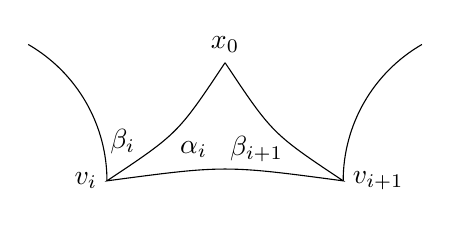
\begin{tikzpicture}
		\draw (0, 1.5) node[above] {$x_0$} .. controls (-0.6, 0.6) .. (-1.5, 0) node[left] (B) {$v_i$}
			.. controls (0, 0.2) .. (1.5, 0) node[right] {$v_{i+1}$}
			.. controls (0.6, 0.6) .. (0, 1.5);
		\node at (-0.4, 0.4) {$\alpha_i$};
		\node at (0.4, 0.4) {$\beta_{i+1}$};
		\draw (-1.5, 0) arc[start angle=0, end angle=60, radius=2];
		\draw (1.5, 0) arc[start angle=180, end angle=120, radius=2];
		\node at (-1.3, 0.5) {$\beta_i$};
	\end{tikzpicture}\end{center}
	于是 Gauss--Bonnet 公式 (定理 \ref{prop:Gauss-Bonnet}) 整理后给出
	\begin{equation}\label{eqn:Siegel-aux-1}
		\mes(P(m,n)) + \angle (v_m x_0 v_n) = \pi - \alpha_m - \beta_n + \sum_{m<i<n} (\pi - \theta(v_i)).
	\end{equation}

	测地凸性确保所有内角落在 $[0, \pi]$ 区间, 所以 \eqref{eqn:Siegel-aux-1} 蕴涵 $\sum_i (\pi - \theta(v_i))$ 单调收敛. 此外 $\angle (v_m x_0 v_n)$ 和 $\mes(P(m,n))$ 也单调收敛. 如固定 $m,n$ 中的任一者而让另一者趋近 $\pm\infty$, 则 \eqref{eqn:Siegel-aux-1} 又蕴涵 $\alpha_m$, $\beta_n$ 分别有极限 $\alpha_-$, $\beta_+$. 兹断言
	\begin{equation}\label{eqn:Siegel-aux-2}
		\alpha_-, \beta_+ \leq \frac{\pi}{2}
	\end{equation}
	基于对称性, 处理 $\beta_+$ 情形即可. 因为 $\mathcal{D}$ 中以 $x_0$ 为原点, 半径有限的任何测地球内仅含有限多个 $v_i$, 必存在无穷多个 $i$ 使得 $d(x_0, v_{i+1}) > d(x_0, v_i)$. 双曲三角形中依然有大边对大角, 证明和经典情形相同, 对这些 $i$ 遂有 $\alpha_i > \beta_{i+1}$. 推论 \ref{prop:angle-defect} 导致 $\alpha_i + \beta_{i+1} \leq \pi$, 故 $\beta_{i+1} \leq \pi/2$. 取 $i \to +\infty$ 便得到 \eqref{eqn:Siegel-aux-2}. 配合 \eqref{eqn:Siegel-aux-1} 即得
	\begin{equation}\label{eqn:Siegel-aux-3}
		\sum_{i = -\infty}^{+\infty} (\pi - \theta(v_i)) \leq \sup_{m,n} \left(\mes(P(m,n)) + \angle(v_m x_0 v_n) \right).
	\end{equation}
	将 \eqref{eqn:Siegel-aux-3} 对所有的顶点列 $\{v_i\}_i$ 求和, 如是得到 \eqref{eqn:Siegel-aux-0}.
	
	现在任取 $D(x_0)$ 的非无穷远顶点 $\eta$, 要求 $\eta$ 非冗余, 亦即 $\theta(\eta) < \pi$. 命题 \ref{prop:angle-sum} 蕴涵
	\begin{equation*}\begin{gathered}
		N := \left| \left\{ \xi \in \partial D(x_0): \xi \sim \eta \right\}\right| \; \in \Z_{\geq 1}, \\
		\sum_{\xi \sim \eta} (\pi - \theta(\xi)) = \left(N - \frac{2}{e(\eta)}\right) \pi.
	\end{gathered}\end{equation*}
	\begin{itemize}
		\item 如 $e(\eta) = 1$, 则 $0 < \theta(\eta) < \pi$ 导致 $N \geq 3$, 从而 $\sum_{\xi \sim \eta} (\pi - \theta(\xi)) \geq \pi$.
		\item 如 $e(\eta) \geq 3$ 则 $\sum_{\xi \sim \eta} (\pi - \theta(\xi)) \geq \frac{\pi}{3}$.
		\item 若 $e(\eta) = 2$ 而 $N \geq 2$, 则 $\sum_{\xi \sim \eta} (\pi - \theta(\xi)) \geq \pi$
		
		因为 $e(\eta)$ 和 $N$ 仅依赖 $\eta$ 的 $\sim$ 类, 与 \eqref{eqn:Siegel-aux-0} 比较可知以上三种顶点至多仅由有限多个 $\sim$ 类组成, 因此其个数有限.
		\item 最后, 若 $e(\eta) = 2$ 而 $N = 1$, 则上式给出 $\theta(\eta) = \pi$, 这种冗余顶点已经排除.
	\end{itemize}
	我们已经证明了 $D(x_0)^*$ 的顶点数目有限, 内角 $\pi$ 的冗余顶点不论. 于是 $\partial D(x_0)^*$ 分解成有限个极大测地线段; 此外再观察到无穷远处的顶点皆尖, 这是因为这些顶点数目有限, 而边界上不可能出现如下图加粗显示的``开口''
	\begin{center}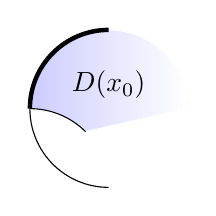
\begin{tikzpicture}
		\fill[draw=white, shading=axis, left color=blue!20, right color=white] (1,1) arc[start angle=0, end angle=180, radius=1] arc[start angle=90, end angle=45, radius=1] --cycle;
		\draw[ultra thick] (0,2) arc[start angle=90, end angle=180, radius=1];
		\draw (-1,1) arc[start angle=180, end angle=270, radius=1];
		\draw (-1,1) arc[start angle=90, end angle=45, radius=1];
		\node[above] at (0,1) {$D(x_0)$};
	\end{tikzpicture}\end{center}
	否则 $D(x_0)$ 的面积将是 $+\infty$. 综之, 对 $D(x_0)$ 应用命题 \ref{prop:parabolic-stabilizer} 即可导出边数有限, 并且得到椭圆点和尖点的所需性质.
\end{proof}

以下设 $x_0$ 非椭圆点. 透过 $\overline{\Gamma}$ 作用诱导的等价关系 $\sim$, 或等价地说 (命题 \ref{prop:pairing-pasting}), 按定义--命题 \ref{prop:side-pairing} 的边配对, 可以对 $D(x_0)^*$ 进行粘合. 以下联系群 $\Gamma$ 的尖点与 Dirichlet 区域 $D(x_0)$ 的无穷远点, 并证明 $X(\Gamma)$ 的紧性.

\begin{theorem}\label{prop:Fuchsian-1st-kind-pasting}
	设 $\Gamma$ 是 $\SL(2, \R)$ 的离散子群, 则 $X(\Gamma)$ 紧当且仅当 $\Gamma$ 是余有限 Fuchs 群. 当此条件成立时, $X(\Gamma) \smallsetminus Y(\Gamma)$ 是有限集, $X(\Gamma)$ 等于 $D(x_0)^*$ 对 $\Gamma$ 作用粘合的产物, 而包含映射
	\[ \left\{ \xi \in D(x_0)^*: \text{无穷远处顶点} \right\} \hookrightarrow \mathcal{C}_\Gamma \]
	将 $X(\Gamma) \smallsetminus Y(\Gamma) = \Gamma \backslash \mathcal{C}_\Gamma$ 等同于 $D(x_0)^*$ 的无穷远点用 $\Gamma$ 或边配对粘合的等价类.
\end{theorem}
\begin{proof}
	首先说明 $X(\Gamma)$ 紧蕴涵 $\Gamma$ 余有限. 根据 \S\ref{sec:X-charts} 对坐标卡的构造, $X(\Gamma) \smallsetminus Y(\Gamma)$ 在 $X(\Gamma)$ 中离散, 故有限. 对于每个 $c \in X(\Gamma) \smallsetminus Y(\Gamma)$, 不失一般性总能假设 $c = \Gamma \infty$, 它附近的坐标邻域遂可取为
	\[ \twomatrix{1}{h\Z}{}{1} \big\backslash \left\{ \tau \in \mathcal{H} : \Im(\tau) > c \right\} \sqcup \{\infty\} , \quad h \in \R_{>0} \]
	的形式, 其中 $c \gg 0$. 此坐标邻域对双曲度量的面积是 $h \cdot \int_c^\infty \frac{\dd y}{y^2} < +\infty$. 因为 $X(\Gamma)$ 紧而尖点数目有限, 这就足以说明 $Y(\Gamma)$ 的双曲面积也有限.

	相对麻烦的是从 $\Gamma$ 余有限推导 $X(\Gamma)$ 紧. 根据命题 \ref{prop:fundamental-domain-paste}, 基本区域按 $\sim$ 或边配对粘合便给出 $Y(\Gamma)$ 和 $X(\Gamma)$. 以下在上半平面 $\mathcal{H}$ 中论证. 定理 \ref{prop:Fuchsian-1st-kind} 已说明 $D(x_0)^*$ 的每个无穷远点都是``尖''的, 并属于 $\mathcal{C}_\Gamma$; 以下说明对每个 $t \in \mathcal{C}_\Gamma$, 存在 $\delta \in \overline{\Gamma}$ 使得 $\delta t$ 是 $D(x_0)^*$ 的无穷远点. 老方法, 对 $\Gamma$ 作适当共轭后, 不妨假设 $t = \infty \in \mathcal{C}_\Gamma$. 枚举 $D(x_0)^*$ 的无穷远点 $t_1, \ldots, t_n$, 过每个 $t_i = \alpha_i^{-1} \infty$ 作相切的极限圆盘 $\alpha_i^{-1} H^\circ_{c_i}$; 此处符号和引理 \ref{prop:horocycle-immersion-aux} 相同. 基于定理 \ref{prop:Fuchsian-1st-kind} 建立的性质, 取 $c_1, \ldots, c_n$ 充分接近 $0$, 可以确保 $D(x_0) \subset \bigcup_{i=1}^n \alpha_i^{-1} H^\circ_{c_i}$.
	
	接着用反证法: 假设 $\{t_1, \ldots, t_n\}$ 和轨道 $\Gamma \infty$ 无交. 根据引理 \ref{prop:horocycle-immersion-aux}, 只要取 $c' \gg 0$, 那么切 $\infty$ 的极限圆盘 $H_{c'}^\circ$ 满足
	\[ \forall \gamma \in \Gamma, \; \forall 1 \leq i \leq n, \quad \gamma\alpha_i^{-1} H_{c_i}^\circ \cap H^\circ_{c'} = \emptyset. \]
	故 $H^\circ_{c'}$ 与所有 $\gamma D(x_0)$ 皆无交; 因为 $D(x_0)$ 是基本区域, 此无可能. 于是我们验证了关于 $X(\Gamma) \smallsetminus Y(\Gamma)$ 的描述.
	
	回顾 \S\ref{sec:X-charts} 对 $\mathcal{C}_\Gamma$ 附近拓扑的定义, 可知``多边形'' $D(x_0)^*$ 视作 $\CC$ 的闭子集, 其拓扑和来自 $\mathcal{H}^* = \mathcal{H} \sqcup \mathcal{C}_\Gamma$ 的诱导拓扑相同, 特别地它是紧的. 综合上述结果, 将 $D(x_0)^*$ 按 $\Gamma$ 粘合后同胚于 $X(\Gamma)$, 从而 $X(\Gamma)$ 也紧.
\end{proof}

\begin{example}
	设 $\Gamma$ 是同余子群. 在 \S\ref{sec:cong-subgroup} 中我们已经说明 $Y(\SL(2,\Z))$ 测度有限. 因为 $(\SL(2,\Z) : \Gamma)$ 有限, $Y(\Gamma)$ 测度亦有限, 相应地 $X(\Gamma)$ 为紧.
\end{example}

\begin{exercise}\label{exo:Fuchsian-1st-generation}
	证明余有限 Fuchs 群必为有限生成群.

	\begin{hint}
		应用练习 \ref{exo:side-pairing-generation}.
	\end{hint}
\end{exercise}

\section{间奏: 可公度性, 算术子群, 四元数}\label{sec:quaternion}
数论或表示论中常见的余有限 Fuchs 群是所谓的\emph{算术子群}, 这是一类与代数群的整点相关的离散子群, 包括熟悉的同余子群和即将介绍的四元数代数情形. 对于算术子群, 从 $Y(\Gamma)$ 到 $X(\Gamma)$ 的过渡是所谓 \emph{Bailey--Borel 紧化}的一个特例, 高维情形一般会产生奇点.

先引进一个群论的基本概念.
\begin{definition}\label{def:commensurable} \index{kegongdu@可公度 (commensurable)} \index[sym1]{approx@$\approx$}
	称群 $\Omega$ 的子群 $H_1, H_2$ 是\emph{可公度的}, 如果 $(H_1: H_1 \cap H_2)$ 和 $(H_2: H_1 \cap H_2)$ 俱有限; 记作 $H_1 \approx H_2$.
\end{definition}

观察到 $H_1 \approx H_2$ 蕴涵 $H_1 \approx H_1 \cap H_2 \approx H_2$. 另外, 如果 $\Omega$ 是 $\Omega'$ 的子群, 那么性质 $H_1 \approx H_2$ 在 $\Omega$ 和 $\Omega'$ 中是等价的.

\begin{lemma}\label{prop:commensurable}
	子群的可公度性 $\approx$ 是一个等价关系.
\end{lemma}
\begin{proof}
	只须验证传递性. 设子群 $H_1, H_2$ 可公度, $H_2, H_3$ 亦可公度. 由嵌入
	\[ H_1 \cap H_2 \big/ H_1 \cap H_2 \cap H_3 \hookrightarrow H_2 \big/ H_2 \cap H_3 \]
	可得
	\[ (H_1 : H_1 \cap H_2 \cap H_3) = (H_1 : H_1 \cap H_2) (H_1 \cap H_2 : H_1 \cap H_2 \cap H_3) < +\infty. \]
	同理有 $(H_3: H_1 \cap H_2 \cap H_3) < +\infty$. 故 $(H_1:H_1 \cap H_3)$ 和 $(H_3:H_1 \cap H_3)$ 俱有限.
\end{proof}

作为例证, 以下说明 $\SL(2,\Z)$ 及其 $\GL(2,\Q)$-共轭可公度. 这既是可公度性的初步例子, 同时又是研究 Hecke 代数前的必要铺垫, 见 \S\ref{sec:Hecke-full-level}.
\begin{proposition}\label{prop:normalize-congruence-subgroup}
	设 $\alpha \in \GL(2,\Q)$.
	\begin{compactenum}[(i)]
		\item $\alpha \SL(2,\Z) \alpha^{-1} \cap \SL(2,\Z)$ 是同余子群,
		\item 作为 $\SL(2,\R)$ 的离散子群, $\alpha \SL(2,\Z) \alpha^{-1} \approx \SL(2,\Z)$.
	\end{compactenum}
\end{proposition}
\begin{proof}
	对于 (i), 只消证明存在 $N \in \Z_{\geq 1}$ 使得 $\alpha^{-1} \Gamma(N) \alpha \subset \SL(2,\Z)$, 因如此则有 $\Gamma(N) \subset \alpha \SL(2,\Z) \alpha^{-1} \cap \SL(2,\Z)$. 设 $\gamma = 1 + N\eta \in \Gamma(N)$, 其中 $\eta \in \Mat_2(\Z)$. 如是则 $\alpha^{-1} \gamma \alpha = 1 + N \alpha^{-1}\eta\alpha$. 取充分可除之正整数 $N_0$ 使得 $\alpha, \alpha^{-1} \in N_0^{-1} \Mat_2(\Z)$, 再取 $N = N_0^2$ 则有 $N \alpha^{-1}\eta\alpha \in \Mat_2(\Z)$. 综之 $\alpha^{-1}\gamma\alpha \in \Mat_2(\Z) \cap \SL(2,\R) = \SL(2,\Z)$.
	
	现在处理 (ii). 由 (i) 已知
	\[ \left( \SL(2,\Z) : \alpha \SL(2,\Z) \alpha^{-1} \cap \SL(2,\Z) \right) < \infty. \]
	用自同构 $x \mapsto \alpha^{-1} x \alpha$ 搬运, 得到
	\[ \left( \alpha^{-1} \SL(2,\Z) \alpha : \SL(2,\Z) \cap \alpha^{-1} \SL(2,\Z) \alpha \right) < \infty; \]
	第二式中以 $\alpha^{-1}$ 代 $\alpha$, 配合第一式便得出 $\alpha \SL(2,\Z) \alpha^{-1} \approx \SL(2,\Z)$.
\end{proof}

假定 $\mathbf{G}$ 是能用 $\Q$ 上多项式方程``代数地''定义的群, 譬如 $\GL(n)$, $\SL(n)$ 或稍后将探讨的 $\Q$ 上四元数代数的单位群; 这样的 $\mathbf{G}$ 称为 $\Q$ 上的线性代数群. 分别记 $\mathbf{G}(\Q)$ 和 $\mathbf{G}(\R)$ 为其有理点和实点所成的群, 那么 $G := \mathbf{G}(\R)$ 自然地带有 Lie 群结构. 我们分三步对 $G$ 或更一般的 Lie 群定义何谓算术子群. \index{suanshuziqun@算术子群 (arithmetic subgroup)}
\begin{enumerate}[(i)]
	\item 根据线性代群的一般理论, 存在能由 $\Q$ 上多项式定义的群嵌入 $\rho: \mathbf{G} \hookrightarrow \GL(n)$. 任选 $\rho$, 那么 $\mathbf{G}(\Z) := \rho^{-1}\GL(n,\Z) \cap \mathbf{G}(\Q)$ 是 $\mathbf{G}(\R)$ 的算术子群.
	\item 更一般地说, 如果 $\mathbf{G}(\R)$ 的离散子群 $\Gamma$ 和来自某个 $\Q$-嵌入 $\rho$ 的 $\mathbf{G}(\Z)$ 可公度, 那么 $\Gamma \subset \mathbf{G}(\R)$ 亦称为算术子群.
	\item 对于一般的 Lie 群 $G$, 若存在 $\Q$ 上的线性代数群 $\mathbf{G}'$ 及如上定义之算术子群 $\Gamma' \subset \mathbf{G}'(\R)$, 连同拓扑群的满射
	\[ f: \mathbf{G}'(\R) \twoheadrightarrow G, \quad \Ker(f)\; \text{为紧群}, \]
	那么 $\Gamma := f(\Gamma')$ 也称为 $G$ 的算术子群.
\end{enumerate}
按定义, 这套手续穷尽了这类 Lie 群 $G$ 的所有算术子群; 形如 (i) 和 (ii) 的算术子群最为常用.

\begin{example}
	定义中取 $\mathbf{G} = \SL(2)$, 它天然地由多项式方程 $\left\{ \twomatrix{a}{b}{c}{d} : ad - bc = 1 \right\}$ 定义, 并且存在当然的嵌入 $\rho: \SL(2) \hookrightarrow \GL(2)$. 那么 $\mathbf{G}(\Z) = \SL(2,\Z)$. 任何满足 $(\SL(2,\Z) : \Gamma)$ 有限的子群 $\Gamma \subset \SL(2,\Z)$ 按上述定义都是算术子群; 特别地, 同余子群必为算术子群. 反观之, 一个自然的问题是: $\SL(2,\Z)$ 中使 $(\SL(2,\Z) : \Gamma)$ 有限的子群是否都是同余子群? 答案是否定的; $\SL(2,\Z)$ 的这一古怪性质早在模形式理论的萌芽时期便引起注意, 史料是 \cite[II.7.11]{KF1}. 一般群的情形请参阅 \cite{BMS67}.
\end{example}

已知 $\SL(2,\R)$ 的算术子群都是余有限 Fuchs 群, 与此相关的技术和结果通称为\emph{化约理论}. 读者在计算 $\SL(2,\Z)$ 的基本区域时已经领教过一些化约手法, 一般情形自然要求更抽象的技术.

在 \S\ref{sec:Y-charts} 末尾谈到了四元数代数和相应的志村曲线, 它们在数论中有深刻的渊源. 现在给予一些较具体, 然而终是蜻蜓点水的描述, 证明大部省去. 这方面的文献有 \cite{Vi80, Voi}. \index{zhicunquxian}

设 $F$ 为域, 所谓 $F$-\emph{代数}是叠架在 $F$-向量空间上的环结构, 使得环的乘法是 $F$-双线性型; 典型例子是 $n \times n$ 矩阵代数 $\Mat_n(F)$. 这里的代数均指含幺结合代数, 未必交换. 代数之间的同态定义为 $F$-线性的环同态. 相关理论见 \cite[第七章]{Li1}.

\begin{definition}\label{def:quaternion-alg}\index{siyuanshudaishu@四元数代数 (quaternion algebra)}
	设 $F$ 是特征 $\neq 2$ 的域, $a, b \in F^\times$. 定义 $F$ 上的\emph{四元数代数} $B := \left( \dfrac{a,b}{F} \right)$ 为以 $1, i, j, k$ 为基的 $4$ 维 $F$-向量空间, 乘法结构由
	\[ 1: \text{乘法幺元}, \quad i^2=a, \quad j^2=b, \quad ij=k=-ji \]
	完全确定. 作为 $F$-代数同构于 $\Mat_2(F)$ 的四元数代数称为是\emph{分裂}的.
\end{definition}

观察到 $\mathbb{H} := \left( \dfrac{-1, -1}{\R} \right)$ 无非是熟悉的 Hamilton 四元数代数.

读者可以验证这般代数结构是良定的, 或者直接在 $\Mat_2$ 里实现它: 取 $X^2 - a \in F[X]$ 的分裂域 $F(\sqrt{a})$, 再定义 $F$-向量空间的映射
\begin{equation}\label{eqn:quat-alg-embedding}\begin{aligned}
	F \oplus Fi \oplus Fj \oplus Fk & \longrightarrow \Mat_2\left(F(\sqrt{a})\right) \\
	x + yi + zj + wk & \longmapsto \twobigmatrix{x + y\sqrt{a}}{z + w\sqrt{a}}{b(z - w\sqrt{a})}{x - y\sqrt{a}}.
\end{aligned}\end{equation}
请读者动手验证这是单射, 右式对乘法封闭, 而且 $\Mat_2\left(F(\sqrt{a})\right)$ 的乘法搬回 $B$ 上正如定义 \ref{def:quaternion-alg} (只消对 $i, j, k$ 的像检查). 因之 $B \to \Mat_2\left(F(\sqrt{a})\right)$ 为 $F$-代数的嵌入. 以下性质都是容易的.
\begin{itemize}
	\item 将基中的 $i,j$ 调换, 代 $k$ 为 $-k$, 可见 $\left( \dfrac{a,b}{F} \right) \simeq \left( \dfrac{b,a}{F} \right)$. 用 $s, t \in F^\times$ 将基作伸缩 $i \leadsto si$, $j \leadsto tj$, $k \leadsto stk$, 可见 $\left( \dfrac{a,b}{F} \right) \simeq \left( \dfrac{s^2a, t^2b}{F} \right)$.
	\item 域变换下的行为也是明白的: 设 $E$ 是 $F$ 的扩域, 按定义遂有 $E$-代数的同构 $\left( \dfrac{a,b}{F} \right) \dotimes{F} E \simeq \left( \dfrac{a,b}{E} \right)$.
	\item 基于 \eqref{eqn:quat-alg-embedding}, 当 $a \in F^{\times 2}$ 时 $\left( \dfrac{a,b}{F} \right) \rightiso \Mat_2(F)$ 故分裂; 当 $b \in F^{\times 2}$ 时 $\left( \dfrac{a,b}{F} \right) \simeq \left( \dfrac{b,a}{F} \right)$ 亦分裂. 特别地, 代数闭域上的四元数代数总是分裂.
\end{itemize}

在一般的四元数代数 $B$ 上定义\emph{共轭}运算
\[ q = x + yi + zj + wk \longmapsto x - yi - zj - wk =: \bar{q}, \]
和从 $B$ 到 $F$ 的多项式映射:
\begin{align*}
	\text{\emph{既约迹}}\quad \Tr(x + yi + zj + wk) & = 2x, \\
	\text{\emph{既约范数}}\quad \mathrm{Nrd}(x + yi + zj + wk) & = x^2 - ay^2 - bz^2 + abw^2.
\end{align*}

例行的操作给出 $q \mapsto \overline{q}$ 是 $F$-线性映射, 服从于 $\overline{q_1 \cdot q_2} = \overline{q_2} \cdot \overline{q_1}$ 和
\begin{gather*}
	 \Tr(q) = q + \bar{q}, \quad \mathrm{Nrd}(q) = q\bar{q} = \bar{q}q, \quad \mathrm{Nrd}(1) = 1, \\
	 \mathrm{Nrd}(q_1 q_2) = \mathrm{Nrd}(q_1) \mathrm{Nrd}(q_2) = \mathrm{Nrd}(q_2 q_1).
\end{gather*}

\begin{proposition}
	设 $B$ 为 $F$ 上的四元数代数, 那么 $q \in B$ 可逆当且仅当 $\mathrm{Nrd}(q) \in F^\times$, 这时 $q^{-1} = \mathrm{Nrd}(q)^{-1} \overline{q}$. 特别地, $B$ 是可除代数的充要条件是 $\mathrm{Nrd}(q) = 0 \iff q = 0$.
\end{proposition}
\begin{proof}
	从 $qq^{-1} = 1$ 可得 $\mathrm{Nrd}(q) \mathrm{Nrd}(q^{-1}) = 1$, 故 $\mathrm{Nrd}(q) \in F^\times$ 而 $q^{-1} = \mathrm{Nrd}(q)^{-1} \overline{q}$. 反过来说, 若 $\mathrm{Nrd}(q) \in F^\times$ 则 $\mathrm{Nrd}(q)^{-1} \overline{q}$ 显然给出 $q$ 的逆.
\end{proof}

定义乘法群 $B^1 := \{q \in B: \text{Nrd}(q)=1 \} \subset B^\times$. 分裂情形下 $B^\times \simeq \GL(2,F)$, 而 $\Tr$ 和 $\text{Nrd}$ 分别对应到方阵的 $\Tr$ 和 $\det$, 从而 $B^1 \simeq \SL(2,F)$.

\begin{example}\label{eg:quaternion-real}
	当 $F = \R$ 时, 将 $(a,b)$ 适当伸缩并重排后可将 $B = \left( \dfrac{a,b}{F} \right)$ 之分类化约到 $(a,b) = (-1,-1)$, $(1, -1)$ 和 $(1, 1)$ 情形, 分类为如下两种.
	\begin{enumerate}
		\item 已知 $\left( \dfrac{-1, -1}{F} \right) \simeq \mathbb{H}$, 此时 \eqref{eqn:quat-alg-embedding} 给出的 $\mathbb{H} \hookrightarrow \Mat_2(\CC)$ 诱导群同构
		\begin{align*}
			B^1 \simeq \mathbb{H}^1 & \stackrel{\sim}{\longrightarrow} \SU(2) \\
			u + vj & \longmapsto \twobigmatrix{u}{v}{-\overline{v}}{\overline{u}}, \quad u,v \in \CC = \R \oplus \R i \hookrightarrow \mathbb{H}.
		\end{align*}
		\item 根据定义 \ref{def:quaternion-alg} 之后的讨论, $\left( \dfrac{1, -1}{F} \right)$ 和 $\left( \dfrac{1, 1}{F} \right)$ 皆分裂, 此时 $B^1 \simeq \SL(2,\R)$.
	\end{enumerate}
\end{example}

以下设域 $F$ 是 $\Q$ 的有限扩张, $\mathfrak{o}_F$ 是 $F$ 中代数整数所成之环; 或者简单起见不妨取 $F=\Q$, $\mathfrak{o}_F = \Z$.

\begin{definition}\label{def:order}\index{xumo@序模 (order)}
	包含于 $F$-代数 $B$ 的\emph{序模}系指一个 $\mathfrak{o}_F$-子模 $\mathcal{O} \subset B$, 使得
	\begin{compactitem}
		\item $\mathcal{O}$ 是有限秩自由 $\mathfrak{o}_F$-模,
		\item $\mathcal{O}$ 同时也是 $B$ 的子环,
		\item $F\mathcal{O} = B$.
	\end{compactitem}
	上述定义适用于任何 $F$-代数 $B$; 如果 $\mathcal{O}$ 对序模的包含关系是极大元, 则称之为极大序模.
\end{definition}

序模的角色是在 $B$ 上定义整结构. 从定义条件立见 $\rank_{\mathfrak{o}_F} \mathcal{O} = \dim_F B$.

\begin{example}
	取 $F = \Q$. 对于 $\left( \dfrac{-1, -1}{\Q}\right)$, 序模的显然候选是 $\Z \oplus \Z i \oplus \Z j \oplus \Z k$. 这不是极大序模: 它包含于 Hurwitz 序模
	\begin{align*}
		\mathcal{O} & := \left\{ \frac{x + yi + zj + wk}{2}: x,y,z,w \in \Z, \; \text{同奇偶性} \right\} \\
		& = \Z \oplus \Z i \oplus \Z j \oplus \Z \cdot \frac{1 + i + j + k}{2}.
	\end{align*}
\end{example}

\begin{exercise}
	试证明上述之 Hurwitz 序模是极大序模.
\end{exercise}

以多项式方程定义在 $F$ 上的对象也可以定义在 $\Q$ 上, 然而每个 $F$-值坐标都得用 $[F:\Q]$ 个 $\Q$-值坐标来代替, 这套手续称为纯量限制或 Weil 限制. 施之于 $F$ 上的四元数代数 $B$, 这无非是将 $B$ 看成 $4[F:\Q]$ 维 $\Q$-代数. 不难想见 $B^1$ 成为 $\Q$ 上的线性代数群, 毕竟一切都是代数地定义在有限维仿射空间上的.

\index{quanshiyu@全实域 (totally real field)}
今起假设 $F$ 是\emph{全实域}, 亦即所有域嵌入 $F \hookrightarrow \CC$ 的像都在 $\R$ 中. 将这些嵌入标为 $\iota_i$, 其中 $0 \leq i < [F: \Q]$. 将 $F$ 写成 $\Q(\theta)$ 之形, 其中 $\theta \in \CC$ 的首一极小多项式为 $P \in \Q[X]$, $F \simeq \Q[X]/(P)$, 那么这些域嵌入透过 $\iota_i(\theta) = \theta_i$ 一一对应于 $P$ 在 $\CC$ 中的根 $\theta_0, \theta_1, \ldots$, 它们都落在 $\R$ 中. 用 $B \dotimes{F, \iota_i} \R$ 表示对域扩张 $F \xrightarrow{\iota_i} \R$ 取张量积, 于是乎有 $\R$-代数的同构
\begin{align*}
	B \dotimes{\Q} \R & \simeq B \dotimes{F} \left( F \dotimes{\Q} \R \right) \simeq B \dotimes{F} \left( \frac{\R[X]}{(P)} \right) \\
	& \simeq B \dotimes{F} \prod_{i=0}^{[F : \Q]-  1} \frac{\R[X]}{(X - \theta_i)} \simeq \prod_{i=0}^{[F:\Q] - 1} \left( B \dotimes{F, \iota_i} \R \right).
\end{align*}

进一步假定存在唯一的 $i$ 使得 $B \dotimes{F, \iota_i} \R$ 分裂, 不妨设 $i=0$. 那么根据例 \ref{eg:quaternion-real}, 当 $i \geq 1$ 时则有 $(B \dotimes{F, \iota_i} \R)^1 \simeq \mathbb{H}^1 \simeq \SU(2)$, 从而有嵌入
\[ (\iota_0, \iota_1, \ldots): B^1 \hookrightarrow (B \dotimes{\Q} \R)^1 \simeq \SL(2,\R) \times \prod_{i=1}^{[F:\Q] - 1} \SU(2). \]
注意到 $B^1$ 是 $\Q$ 上的线性代数群, 另记为 $\mathbf{G}'$, 那么嵌入的右端是 Lie 群 $\mathbf{G}'(\R)$; 投影同态 $\mathbf{G}'(\R) \xrightarrow{\pi} \SL(2, \R)$ 的核是紧群. 合成同态 $\pi \circ (\iota_0, \iota_1, \ldots)$ 无非是对应 $\iota_0$ 的群嵌入
\begin{equation}\label{eqn:B-SL2}
	B^1 \hookrightarrow (B \dotimes{F, \iota_0} \R)^1 \simeq \SL(2,\R).
\end{equation}
不难验证 $\mathcal{O} \cap B^1$ 对之的像是 $\SL(2,\R)$ 的算术子群. 这是从序模构造算术子群的手法.

\begin{example}
	取 $F = \Q$, $B = \Mat_2(\Q)$, 序模为 $\mathcal{O} := \Mat_2(\Z)$. 那么 $\mathcal{O} \cap B^1$ 透过 \eqref{eqn:B-SL2} 在 $\SL(2,\R)$ 中的像无非是熟知的 $\SL(2,\Z)$.
\end{example}

作为另一则示范, 今参照 \cite[\S 5]{KV03} 取 $F=\Q$, $B = \left( \dfrac{2, -3}{\Q} \right)$. 例 \ref{eg:quaternion-real} 表明 $B \dotimes{\Q} \R \simeq \left( \dfrac{1, -1}{\R} \right)$ 分裂. 取序模为
\[ \mathcal{O} := \Z \oplus \Z\cdot \dfrac{i + k}{2} \oplus \Z\cdot \dfrac{1 + j}{2} \oplus \Z k. \]
它实际是一个极大序模. 嵌入 $B \hookrightarrow \Mat_2(\R)$ 取为合成
\[ B \xrightarrow{\eqref{eqn:quat-alg-embedding}} \Mat_2\left(\Q(\sqrt{2})\right) \xrightarrow{\Q(\sqrt{2}) \; \subset \; \R} \Mat_2(\R). \]
所得的算术子群记作 $\Gamma^6_0(1) \subset \SL(2,\R)$. 以下讨论它的 Dirichlet 区域, 见 \S\ref{sec:Dirichlet-domain}.

记 $2j-k \in B^\times$ 在 $\mathcal{H}$ 上的作用为 $\pi_6$. 定义
\[ a := \dfrac{(-2\sqrt{2} + 3)\sqrt{-3}}{3},\; b := \dfrac{(4\sqrt{2}-5)(3 + 2\sqrt{-3})}{21},\; c := \dfrac{(\sqrt{2}-1)(1+\sqrt{-2})}{3}. \]
取 $b', c'$ 为 $b,c$ 对虚数轴的镜射, 再取 $d' := \pi_6(b)$, $d := \pi_6(b')$, $e := \pi_6(a)$. 那么 $\Gamma^6_0(1)$ 在 $\mathcal{H}$ 上作用的 Dirichlet 区域可以取为以点 $a,b,c,d,e,d',c',b'$ 为顶点的测地多边形 (如图).

\begin{figure}[h]
	\centering
	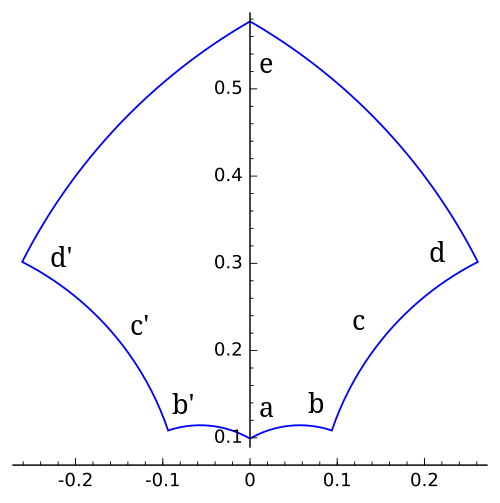
\includegraphics[width=0.4\textwidth]{quat-domain.png}
	\caption{$\Gamma^6_0(1)$ 的一个基本区域, 以 SageMath 软件绘制.}
\end{figure}

该基本区域的样貌与同余子群情形显著不同: 它没有无穷远点, 因而为紧, 由此推得 $Y(\Gamma^6_0(1)) = X(\Gamma^6_0(1))$ 已然是紧 Riemann 曲面. 推而广之, 以下命题断言来自 $B^1$ 的算术子群皆无尖点.

\begin{proposition}\label{prop:B-no-parabolic}
	设 $B = \left( \dfrac{2, -3}{\Q} \right)$, 那么 $B$ 非分裂. 若 $\Gamma \subset \SL(2,\R)$ 是来自 $B^1$ 的算术子群, 则 $\Gamma$ 不含抛物元; 特别地, $\Gamma$ 无尖点.
\end{proposition}
\begin{proof}
	我们先说明任何 $q \in B^1 \smallsetminus \{\pm 1\}$ 都不可能透过 \eqref{eqn:B-SL2} 映为 $\SL(2,\R)$ 的抛物元. 记 $q$ 在 $\SL(2,\R)$ 中的像为 $\gamma$. 若 $\gamma$ 为抛物元, 那么 $\Tr(\gamma)^2 = 4$ 蕴涵 $q = \pm 1 + yi + zj + wk$, 而 $\text{Nrd}(q) = \det(\gamma)=1$ 蕴涵 $-2y^2 + 3z^2 - 6w^2 = 0$ 有非平凡的有理解; 行换元 $y \leadsto 3y$, $z  \leadsto 2z$ 后这等价于 $-3y^2 + 2z^2 = w^2$ 有非平凡有理解. 更可进一步假设 $y,z,w \in \Z$ 无 $\neq \pm 1$ 的公因子. 因为 $2$ 非 $\bmod\; 3$ 的二次剩余, 故
	\[ 2z^2 \equiv w^2 \pmod 3 \implies z \equiv 0 \pmod 3 \implies z \equiv w \equiv 0 \pmod 3, \]
	于是 $y^2 = \frac{w^2 - 2z^2}{-3}$ 也被 $3$ 整除, 矛盾.
	
	特别地, $\Gamma$ 作为 $\mathcal{O} \cap B^1$ 的像不可能包含抛物元. 假如 $B$ 分裂, 则 $B^1 \simeq \SL(2,\Q) \supset \twomatrix{1}{\Q}{}{1}$ 将包含 $\SL(2,\R)$ 的抛物元, 亦矛盾. 尖点之阙如则是定义 \ref{def:cusp-discrete-subgroup} 的直接结论.
\end{proof}

\begin{remark}
	A.\ Weil 对典型群的分类蕴涵以下推论: 精确到可公度性, $\SL(2,\R)$ (或 $\PSL(2, \R)$) 的所有算术子群 $\Gamma$ (或 $\overline{\Gamma}$) 都透过 \eqref{eqn:B-SL2} 来自某个全实域 $F$, 只对一个嵌入 $F \hookrightarrow \R$ 分裂的四元数 $F$-代数 $B$, 以及序模 $\mathcal{O} \subset B$. 相关细节和 $\overline{\Gamma}$ 的基本区域的性质可参阅 \cite[\S 38]{Voi}. 一个事实是 $B$ 非分裂时 $Y(\Gamma)$ 必为紧. 命题 \ref{prop:B-no-parabolic} 已经实算了一个具体例子.
\end{remark}

志村曲线的众多妙用之一是构造两个二维紧 Riemann 流形, 使之不等距但等谱; 后者意谓两者的 Laplace--Beltrami 算子有相同的特征值 (计重数), 见 \cite[IV.3.E]{Vi80}. 为此须运用 $\Q$ 的二次扩张上的四元数代数和 Selberg 迹公式, 这已经逾越本书范围.


\section{整权模形式的一般定义}\label{sec:modular-form-general}
模形式在同余子群情形的定义 \ref{def:modular-form} 可以毫不困难地推及任何余有限 Fuchs 群 $\Gamma$. 相关讨论几乎与 \S\ref{sec:modular-form-cong} 平行.

择定权 $k \in \Z$. 先前关于 $Y(\Gamma)$ 和 $X(\Gamma)$ 的种种构造仅涉及 $\overline{\Gamma}$ 的结构. 一旦考虑定义 \ref{def:bar-action} 中 $\Gamma$ 的右作用 $f \mapsto f \modact{k} \gamma$, 由于 $f \modact{k} (-1) = (-1)^k f$, 当 $k \notin 2\Z$ 时单看 $\overline{\Gamma}$ 是不够的. 我们将需要以下概念.

\begin{definition}[正则尖点]\label{def:regular-cusp} \index{jiandian!正则 (regular)}
	设 $-1 \notin \Gamma$ 而 $t \in \mathcal{C}_\Gamma$. 存在 $\alpha \in \SL(2, \R)$ 使得 $t = \alpha\infty$, 从而在 $\PSL(2,\R)$ 中
	\[ \alpha^{-1} \overline{\Gamma}_t \alpha = \lrangle{\twomatrix{1}{h}{}{1}}, \quad h \in \R_{>0}; \]
	见 \eqref{eqn:cusp-width}, 该处的 $\alpha$ 相当于这里的 $\alpha^{-1}$. 现将上式提升到 $\SL(2,\R)$ 中来考察. 因为 $-1 \notin \Gamma$, 以下两种情形必居其一:
	\begin{compactitem}
		\item 若 $\twomatrix{1}{h}{}{1} \in \alpha^{-1} \Gamma_t \alpha$, 称相应的尖点为\emph{正则}的;
		\item 若 $-\twomatrix{1}{h}{}{1} \in \alpha^{-1} \Gamma_t \alpha$, 称相应的尖点为\emph{非正则}的.
	\end{compactitem}
\end{definition}

\begin{exercise}
	验证以上定义不依赖于 $\alpha$ 的选取, 而且只关乎 $t$ 的 $\Gamma$ 轨道, 换言之只依赖于 $X(\Gamma)$ 中相应的尖点.
\end{exercise}

\begin{exercise}\label{exo:regular-cusp}
	证明当 $N \geq 3$ (或 $N \geq 5$) 时, $\Gamma(N)$ (或 $\Gamma_1(N)$) 的所有尖点都正则.
	
	\begin{hint}
		对于 $\Gamma(N)$, 考虑由 $\alpha \infty \in \Q^*$ 给出的尖点, 其中 $\alpha \in \SL(2,\Z)$. 由 $\alpha^{-1} \Gamma(N) \alpha = \Gamma(N)$ 可见 $\alpha^{-1} \Gamma(N)_{\alpha\infty} \alpha = \Gamma(N)_\infty$, 而条件蕴涵 $\Gamma(N)_\infty = \twomatrix{1}{N\Z}{}{1}$. 对于 $\Gamma_1(N)$, 若存在非正则极点, 则存在抛物元素 $\gamma \in \Gamma_1(N)$ 使得 $\Tr(\gamma) = -2$, 这将蕴涵 $N \mid 4$.
	\end{hint}
\end{exercise}

非正则尖点的实例将在例 \ref{eg:Gamma14-genus} 给出.

对于全纯函数 $f: \mathcal{H} \to \CC$, 假若 $f$ 有周期 $x > 0$, 亦即 $f(\tau + x) = f(\tau)$, 则可以按 Laurent 级数展开
\[ f(\tau) = \sum_{n \in \Z} a_n q_x^n, \quad q_x := e^{2\pi i\tau/x}. \]
一如定义 \ref{def:cusp-vanishing}, 我们按展开中是否仅有 $n \geq 0$ (或 $n > 0$, 或至多有限个 $n < 0$) 的非零项, 称 $f$ 在 $\infty$ 处全纯 (或消没, 或亚纯). 这些性质在平移变换 $f(\tau) \leadsto f(\tau + b)$ 下并不改变 ($b \in \R$). 此一展开式称为 Fourier 展开, 系数称为 Fourier 系数. \index{Fourier 系数}

对每个 $t = \alpha\infty \in \mathcal{C}_\Gamma$, 其中 $\alpha \in \SL(2,\R)$, 我们希望探讨 $f \modact{k} \alpha$ 在 $\infty$ 处的 Fourier 展开. 为此, 我们取 $f \modact{k} \alpha$ 的周期
\[ x := \min\left\{ x' \in \R_{>0} : \twobigmatrix{1}{x'}{}{1} \in \alpha^{-1}\Gamma_t \alpha \right\}, \]
此时
\[ \alpha^{-1} \Gamma_t \alpha \cap \twobigmatrix{1}{*}{}{1} = \twobigmatrix{1}{x\Z}{}{1}. \]
上式的 $x$ 未必等于定义 \ref{def:regular-cusp} 中的 $h$, 因为后者是在 $\PSL(2,\R)$ 中来考虑的. 在此请读者验证: 若 $-1 \in \Gamma$ 则 $x=h$; 若 $-1 \notin \Gamma$ 则
\begin{equation}\label{eqn:x-vs-h}
	x = \begin{cases}
		h, & t \;\text{为正则尖点} \\
		2h, & t \;\text{非正则尖点}.
\end{cases}\end{equation}

\begin{definition}\label{def:modular-form-gen}
	\index{moxingshi} \index{jiandianxingshi} \index{ji} \index{quan}
	设 $\Gamma$ 为余有限 Fuchs 群, $k \in \Z$. 对于全纯函数 $f: \mathcal{H} \to \CC$, 若
	\begin{enumerate}[(i)]
		\item 对所有 $\gamma \in \Gamma$ 皆有 $f \modact{k} \gamma = f$,
		\item 对每个 $t = \alpha\infty \in \mathcal{C}_\Gamma$, 其中 $\alpha \in \SL(2,\R)$ 者, $f\modact{k}\alpha$ 在 $\infty$ 处全纯,
	\end{enumerate}
	则称 $f$ 是权为 $k$, 级为 $\Gamma$ 的\emph{模形式}. 若进一步在 (ii) 中要求 $f \modact{k} \alpha$ 在 $\infty$ 处消没, 则称 $f$ 是\emph{尖点形式}. 它们构成的 $\CC$-向量空间分别记为 $M_k(\Gamma)$ 和 $S_k(\Gamma)$. 若将 $f$ 在 $\mathcal{H}$ 上及在条件 (ii) 中的全纯条件放宽为亚纯, 相应地便得到\emph{亚纯模形式}的概念.
	\index{moxingshi!亚纯 (meromorphic)}
\end{definition}

尖点处的条件 (ii) 只依赖于 $t$ 的 $\Gamma$-轨道, 或者说只依赖于双陪集 $\Gamma \cdot \alpha \cdot \Stab_{\SL(2,\R)}(\infty)$, 道理与定义--命题 \ref{def:Const} 前的讨论类似, 细说如下:
\begin{compactitem}
	\item 基于条件 (i), 将 $\alpha$ 左乘以 $\Gamma$ 的元素不改变 $f \modact{k} \alpha$.
	\item 设 $\beta \in \Stab_{\SL(2,\R)}(\infty)$. 按引理 \ref{prop:stab-cusp} 表之为
	\[ \beta = \twobigmatrix{a}{b}{}{a^{-1}}, \quad \beta: \tau \mapsto a^2 \tau + ab. \]
	变 $\alpha$ 为 $\alpha\beta$ 相当于变 $g := f \modact{k} \alpha$ 为 $g^* := g \modact{k} \beta: \tau \mapsto a^{-k} g(a^2 \tau + ab)$. 又由于
	\[ \beta^{-1} \twobigmatrix{1}{x}{}{1} \beta = \twobigmatrix{a^{-1}}{-b}{}{a} \twobigmatrix{1}{x}{}{1} \twobigmatrix{a}{b}{}{a^{-1}} = \twobigmatrix{1}{a^{-2} x}{}{1}, \]
	所论的周期 $x$ 相应地变为 $a^{-2} x$. 综之,
	\begin{align*}
		g^*(\tau) & = a^{-k} \sum_n a_n \exp\left( 2\pi i n \cdot \frac{a^2 \tau + ab}{x} \right) \\
		& = a^{-k} \sum_n a_n \exp\left( 2\pi i n \cdot \frac{\tau}{a^{-2}x} \right) \exp\left( 2\pi i n x^{-1} ab \right) \\
		& = a^{-k} \sum_n a_n \exp\left( 2\pi i n x^{-1} ab \right) q_{a^{-2}x}^n.
	\end{align*}
	故条件 (ii) 中相应的全纯和消没性质亦不变. 进一步, Fourier 展开的常数项只差一个因子 $a^{-k}$.
\end{compactitem}

\begin{remark}\label{rem:common-cusps}
	今后将反复运用以下观察: 模形式 $f \in M_k(\Gamma)$ 或 $S_k(\Gamma)$ 的定义中, (i) 的 $\Gamma$-不变性当然和 $\Gamma$ 的选择密切相关; 条件 (ii) 则只牵涉 $\mathcal{C}_\Gamma$. 作为推论, 给定余有限 Fuchs 群 $\Gamma, \Gamma' \subset \SL(2,\R)$, 当两者可公度时 (定义 \ref{def:commensurable}), 条件 (ii) 对 $\Gamma$ 和对 $\Gamma'$ 是同一的, 缘由在于命题 \ref{prop:common-cusps} 确保
	\[ \mathcal{C}_\Gamma = \mathcal{C}_{\Gamma \cap \Gamma'} = \mathcal{C}_{\Gamma'}. \]
	作为推论, 当 $(\Gamma:\Gamma') < +\infty$ 时 $M_k(\Gamma) = M_k(\Gamma')^{\Gamma\text{-不变}}$, $S_k(\Gamma) = S_k(\Gamma')^{\Gamma\text{-不变}}$.
\end{remark}

\begin{remark}
	如果 $\Gamma$ 没有尖点 (例如 \S\ref{sec:quaternion} 提及的志村曲线情形), 定义 \ref{def:modular-form-gen} 的条件 (ii) 便是空的. 如此一来, 模形式和模曲线 $X(\Gamma)$ 的定义在无尖点情形是大大地简化了; 另一方面, 无尖点则无 Fourier 展开, 这对模形式的深入研究会带来更大的挑战.
\end{remark}

以下结果对于验证一个函数是否为模形式极为方便, 有时甚且是必要的.
\begin{proposition}\label{prop:automatic-holomorphy}
	令 $\Gamma$ 为余有限 Fuchs 群, $k \in \Z$. 设全纯函数 $f: \mathcal{H} \to \CC$ 满足
	\begin{compactitem}
		\item 定义 \ref{def:modular-form-gen} 中的 $\Gamma$-不变性 (i),
		\item 存在尖点 $t = \alpha\infty \in \mathcal{C}_\Gamma$ 和相应的 Fourier 展开 $f \modact{k} \alpha = \sum_{n \geq 0} a_n q_x^n$, 使得存在依赖于 $f, t$ 的常数 $M \geq 0$ 使得 $|a_n| \ll n^M$,
	\end{compactitem}
	那么 $f$ 在 $\Gamma$ 的每个尖点处都全纯, 因而 $f \in M_k(\Gamma)$.
\end{proposition}
\begin{proof}
	取共轭 $\Gamma \leadsto \alpha^{-1}\Gamma \alpha$ 和 $f \leadsto f \modact{k} \alpha$, 可化约到 $\infty \in \mathcal{C}_\Gamma$ 而 $\alpha = 1$ 的情形. 我们希望证明当
	\[ \beta = \twomatrix{a}{b}{c}{d} \in \SL(2,\R), \quad t = \beta\infty \in \mathcal{C}_\Gamma \smallsetminus \{\infty\}, \]
	时, 函数 $g := f \modact{k} \beta$ 在 $\infty$ 处全纯. 观察到 $t \neq \infty$ 蕴涵 $c \neq 0$, 而
	\[ g(\tau) = (c\tau + d)^{-k} \sum_{n \geq 0} a_n Q_x^n, \quad Q_x := \exp\left(2 \pi ix^{-1} \cdot \dfrac{a\tau + b}{c\tau + d} \right). \]
	设 $g(\tau)$ 在 $\infty$ 处的 Laurent 展开为 $\sum_{n \in \Z} b_n q_y^n$, 其中 $q_y := \exp(2\pi i y^{-1} \tau)$, $y \in \R_{>0}$. 根据复变函数论的常识 (如 \cite[\S 4.2, 定理 1]{TW06}), 仅须证明 $\lim_{\tau \to \infty} q_y g(\tau) = 0$ 即足. 注意到当 $\Im(\tau) \to +\infty$ 而 $0 \leq \Re(\tau) \leq y$ 时,
	\begin{compactitem}
		\item $q_y$ 作为 $\Im(\tau)$ 的函数按指数衰减;
		\item $(c\tau + d)^{-k}$ 至多按 $\Im(\tau)$ 的多项式增长.
	\end{compactitem}
	上述估计对 $\Re(\tau)$ 还是一致的. 故仅须证明 $\sum_{n \geq 0} a_n Q_x^n$ 相对于 $\Im(\tau)$ 至多呈多项式增长.
	
	设 $\tau = u + iv$, 其中 $v > 0$ 而 $0 \leq u \leq y$. 以 $\lceil M \rceil$ 代 $M$ 可设 $M \in \Z_{\geq 0}$. 根据引理 \ref{prop:fractional-transform-sign},
	\begin{align*}
		\sum_{n \geq 0} a_n Q_x^n & \ll \sum_{n \geq 0} n^M |Q_x|^n, \\
		|Q_x| & = \exp\left( -2\pi x^{-1} \Im\left(\dfrac{a\tau+b}{c\tau+d}\right) \right) \\
		& = \exp\left( -2\pi x^{-1} |c\tau + d|^{-2} v \right).
	\end{align*}
	兹断言存在实系数多项式 $P$ 使得
	\[ \sum_{n \geq 0} n^M |Q_x|^n = \dfrac{P(|Q_x|)}{(1 - |Q_x|)^{M+1}}. \]
	引入变元 $q$, 在收敛范围 $|q|<1$ 内考虑 $\sum_{n \geq 0} q^n = (1-q)^{-1}$, 反复求导得 $\sum_{n \geq h} \binom{n}{h} q^{n-h} = (1-q)^{-h-1}$, 如是可导出以上性质.
	
	当 $v \to \infty$ 时 $Q_x \to e^{2\pi ix^{-1} t}$, 故 $P(|Q_x|)$ 有极限. 为了得出 $\sum_{n \geq 0} n^M |Q_x|^n$ 对 $v = \Im(\tau)$ 至多按多项式增长, 只要证明存在 $N > 0$ 使得
	\[ \lim_{v \to \infty} \dfrac{1}{v^N \left( 1 - |Q_x| \right) } = 0, \]
	而且该极限对 $u \in [0, y]$ 是一致的. 当 $v \to +\infty$ 时,
	\begin{align*}
		1 - |Q_x| & =  1 - \exp\left( -2\pi x^{-1} |c\tau + d|^{-2} v \right) \\
		& = 2\pi x^{-1} |c\tau + d|^{-2} v \left( 1 + o(1) \right).
	\end{align*}
	因为 $u \in [0, y]$, 故 $v \to +\infty$ 时 $|c\tau + d|^2 = (cu+d)^2 + (cv)^2 \sim c^2 v^2$. 于是取 $N \geq 2$ 即有
	\[ v^N \left( 1 - |Q_x| \right) \approx 2\pi x^{-1}c^{-2} v^{N-1} (1 + o(1)) \xrightarrow{v \to +\infty} \infty. \]
	相关估计对 $u$ 显然是一致的. 证毕.
\end{proof}

我们将在定理 \ref{prop:Hecke-bound} 推导上述结果在 $f \in S_k(\Gamma)$ 时的逆命题: $f$ 在尖点的 Fourier 系数至多按 $n^{k/2}$ 增长. 当 $\Gamma$ 是同余子群时, 可进一步对所有 $f \in M_k(\Gamma)$ 得到 $n^k$ 的估计, 见定理 \ref{prop:Hecke-bound-cong}.

\section{Petersson 内积}\label{sec:Petersson}
选定余有限 Fuchs 群 $\Gamma \subset \SL(2,\R)$, 本节主旨是在 $S_k(\Gamma)$ 上定义一个标准的 Hermite 内积. 所谓 $\CC$-向量空间 $S$ 上的 Hermite 内积, 是指一个服从下述条件的映射 $\innerp{\cdot}{\cdot}: S \times S \to \CC$
\begin{compactitem}
	\item $\innerp{ax+by}{z} = a\innerp{x}{z} + b\innerp{y}{z}$, 其中 $a,b \in \CC$;
	\item $\innerp{x}{y} = \overline{\innerp{y}{x}}$;
	\item $\innerp{x}{x} \geq 0$, 等号成立当且仅当 $x=0$.
\end{compactitem}

按注记 \ref{rem:Y-metric}, 我们选定 $\Gamma$ 的基本区域 $\mathcal{F}$ 使得 $\partial \mathcal{F}$ 为零测集, 比方说 Dirichlet 区域, 以其双曲测度来定义 $\mes(Y(\Gamma)) < +\infty$. 进一步, 可以谈论任意可测函数 $\varphi: Y(\Gamma) \to \CC$ 是否可积, 及其积分的值; 相应的测度且记为 $\mu$. 对此可有两种等价的观点:
\begin{compactitem}
	\item 扣掉 $\Gamma$ 的椭圆点 (可数多个, 离散) 得到 $\Gamma$-不变开子集 $\mathcal{H}' \subset \mathcal{H}$, 相应地有 $Y(\Gamma)' \subset Y(\Gamma)$. 于是 $Y'(\Gamma)$ 是 $\mathcal{H}'$ 对自由群作用的商, 从 $\mathcal{H}'$ 继承 Riemann 流形结构. 本节记相应的测度为 $\mu$.
	\item 将 $\varphi$ 拉回 $\mathcal{H}$, 再限制到 $\mathcal{F}$ 上对双曲测度积分, 亦即
	\[ \int_{Y(\Gamma)} \varphi(\tau) \dd\mu(\tau) = \int_{\mathcal{F}} \varphi(\tau) \dfrac{\dd x \wedge \dd y}{y^2}, \qquad \tau = x + iy. \]
\end{compactitem}
既然 $\mes(Y(\Gamma)) < +\infty$, 任何 $Y(\Gamma)$ 上的有界可测函数都可积.

以下选定 $k \in \Z$ 以定义模形式空间 $M_k(\Gamma) \supset S_k(\Gamma)$; 它们都是有限维 $\CC$-向量空间 (推论 \ref{prop:M-finiteness}, 定理 \ref{prop:dimension-formula-odd}).

\begin{definition-theorem}\label{def:Petersson} \index{Petersson 内积} \index[sym1]{(fg)@$\innerPet{f}{g}$}
	设 $f, g \in M_k(\Gamma)$, 其中至少有一者属于 $S_k(\Gamma)$, 则
	\[ \innerPet{f}{g} := \dfrac{1}{\mes(Y(\Gamma))} \int_{Y(\Gamma)} f(\tau) \overline{g(\tau)} \Im(\tau)^k \dd\mu(\tau) \]
	是良定的; 这给出 $S_k(\Gamma)$ 上的 Hermite 内积, 称为 \emph{Petersson 内积}.
\end{definition-theorem}
\begin{proof}
	定义连续函数 $\varphi(\tau) = \varphi[f,g](\tau) := f(\tau) \overline{g(\tau)} \Im(\tau)^k$. 首务是证 $\varphi = \varphi[f,g]$ 下降为 $Y(\Gamma)$ 上的函数. 对任意 $\gamma \in \GL(2,\R)^+$, 应用定义 \ref{def:bar-action} 和引理 \ref{prop:fractional-transform-sign} 来改写
	\begin{equation}\label{eqn:Petersson-aux} \begin{aligned}
		\varphi[f,g](\gamma\tau) & = (f \modact{k} \gamma)(\tau) \overline{(g \modact{k} \gamma)(\tau)} \det(\gamma)^{-k} j(\gamma, \tau)^k \overline{j(\gamma, \tau)}^k \cdot \\
		& \cdot \Im(\tau)^k (\det\gamma)^k |j(\gamma,\tau)|^{-2k} \\
		& = (f \modact{k} \gamma)(\tau) \overline{(g \modact{k} \gamma)(\tau)} \Im(\tau)^k \\
		& = \varphi\left[ f \modact{k} \gamma, \; g \modact{k} \gamma \right](\tau).
	\end{aligned}\end{equation}
	若取 $\gamma \in \Gamma$ 便得到 $ \varphi(\gamma\tau) = \varphi(\tau)$.

	视 $\varphi$ 为 $Y(\Gamma)$ 上的函数, 则连续性自动成立. 现在考量 $\varphi$ 在任意 $t = \alpha\infty \in \mathcal{C}_\Gamma$ 附近的性状, 其中 $\alpha \in \SL(2,\R)$. 根据 \eqref{eqn:Petersson-aux},
	\[ \varphi(\alpha\tau) = (f \modact{k} \alpha)(\tau) \overline{(g \modact{k} \alpha)(\tau)} \Im(\tau)^k \]
	当 $y := \Im(\tau) \to +\infty$ 时 $y^k$ 呈多项式增长, 而从模形式的 Fourier 展开可知 $f \modact{k} \alpha$ 和 $g \modact{k} \alpha$ 在 $y \mapsto +\infty$ 时皆有界, 而且其中属于 $S_k(\Gamma)$ 者按 $|\exp(2\pi i\tau/x)| = \exp(-2\pi y/x)$ 递减到零, 这里 $x \in \R_{>0}$. 指数支配多项式, 故 $\varphi(\alpha\tau) \to 0$. 这就将 $\varphi$ 连续地按零延拓到 $X(\Gamma)$ 上, 而 $X(\Gamma)$ 紧导致 $|\varphi|$ 有界, 因此 $\int_{Y(\Gamma)} |\varphi| < + \infty$.
	
	显然 $\innerPet{f}{g} = \overline{\innerPet{g}{f}}$. 设 $f \in S_k(\Gamma)$, 从 $f$ 的连续性易见 $\innerPet{f}{f} = 0 \iff \varphi[f,f] = 0 \iff f=0$. 综之, $\innerPet{\cdot}{\cdot}$ 确实给出 $S_k(\Gamma)$ 上的 Hermite 内积.
\end{proof}

证明中定义的函数 $\varphi[f, g]$ 满足 $|f(\tau)| \Im(\tau)^{k/2} = \left|\varphi[f,f](\tau)\right|^{1/2}$, 它给出如下的副产品.

\begin{proposition}\label{prop:Hecke-bound-prep}
	当 $f \in S_k(\Gamma)$ 时 $|f(\tau)| \Im(\tau)^{k/2}$ 是 $\mathcal{H}$ 上的有界函数.
\end{proposition}

\begin{exercise}
	以下是命题 \ref{prop:Hecke-bound-prep} 之逆. 对 $f \in M_k(\Gamma)$ 定义 $\psi[f](\tau) := |f(\tau)| \Im(\tau)^{k/2}$. 证明 $\psi[f]$ 有界蕴涵 $f \in S_k(\Gamma)$.
	
	\begin{hint}
		对于 $t = \alpha \infty \in \mathcal{C}_\Gamma$, 注意到 $\psi[f \modact{k} \alpha](\tau) = \psi[f](\alpha\tau)$, 它在 $\Im(\tau) \to +\infty$ 时有界导致 $f \modact{k} \alpha$ 在 $\infty$ 处消没.
	\end{hint}
\end{exercise}


必要时以 $\innerPet{f}{g}^\Gamma$ 来标记 Petersson 内积系相对于 $\Gamma$ 而言. 下一命题解释因子 $\mes(Y(\Gamma))^{-1}$ 的功能: 它表明当 $\Gamma$ 在一个可公度类中变动时, 上标 $\Gamma$ 其实可以略去.

\begin{proposition}\label{prop:Pet-indep}
	假设离散子群 $\Gamma, \Gamma' \subset \SL(2,\R)$ 可公度, 那么 $\Gamma$ 是余有限 Fuchs 群当且仅当 $\Gamma'$ 是余有限 Fuchs 群.
	
	如果 $\Gamma$ 是余有限 Fuchs 群而子群 $\Gamma'$ 满足 $(\Gamma : \Gamma') < +\infty$, 则有自然的包含关系
	\[ S_k(\Gamma) \subset S_k(\Gamma'), \quad M_k(\Gamma) \subset M_k(\Gamma'). \]
	进一步,
	\[ f \in M_k(\Gamma), \; g \in S_k(\Gamma) \implies  \innerPet{f}{g}^\Gamma =  \innerPet{f}{g}^{\Gamma'}. \]
\end{proposition}
\begin{proof}
	对于第一个断言, 按定义 \ref{def:commensurable} 容易化约到 $\Gamma' \subset \Gamma$ 而 $(\Gamma : \Gamma') < +\infty$ 之情形. 取定 $\overline{\Gamma}$ 的基本区域 $\mathcal{F}$ 使 $\partial \mathcal{F}$ 为零测集, 例如 Dirichlet 区域. 根据命题 \ref{prop:fundamental-domain-sub}, 可取 $\overline{\Gamma'}$ 的基本区域 $\mathcal{F}'$ 为 $(\overline{\Gamma} : \overline{\Gamma'})$ 份 $\mathcal{F}$ 的 $\overline{\Gamma}$-平移之并, 那么 $\partial \mathcal{F}'$ 仍为零测集. 测度的定义遂给出
	\[ \mes(Y(\Gamma')) = \mes(\mathcal{F}') = (\overline{\Gamma} : \overline{\Gamma'}) \mes(\mathcal{F}) = (\overline{\Gamma} : \overline{\Gamma'}) \mes(Y(\Gamma)). \]
	所以 $\Gamma$ 是余有限 Fuchs 群当且仅当 $\Gamma'$ 亦然.
	
	今起设 $\Gamma$ 是余有限 Fuchs 群, 且设 $(\Gamma : \Gamma') < +\infty$ 如上. 模形式空间的包含关系已经在注记 \ref{rem:common-cusps} 中说明. 照例记 $\tau = x + iy$. 对于 $f \in M_k(\Gamma)$ 和 $g \in S_k(\Gamma)$, 定义--定理 \ref{def:Petersson} 的证明中已说明函数 $f(\tau)\overline{g(\tau)}y^k$ 对 $\Gamma$ 作用不变, 从而
	\[ \int_{\mathcal{F}'} f(\tau) \overline{g(\tau)} y^k \dfrac{\dd x \dd y}{y^2} = (\overline{\Gamma} : \overline{\Gamma'}) \int_{\mathcal{F}} f(\tau) \overline{g(\tau)} y^k \dfrac{\dd x \dd y}{y^2} \]
	配合以上关于测度的讨论即可完成最后一条断言的证明.
\end{proof}

以下来比较共轭子群的 Petersson 内积, 它将在 Hecke 算子的研究中用上.
\begin{lemma}\label{prop:transport-conjugation}
	设 $\delta \in \GL(2,\R)^+$, 则有复向量空间的同构
	\[\begin{tikzcd}[row sep=tiny]
		S_k(\Gamma) \arrow[r, "\sim"] \arrow[phantom, d, "\subset" sloped] & S_k(\delta^{-1} \Gamma \delta) \arrow[phantom, d, "\subset" sloped] \\
		M_k(\Gamma) \arrow[r, "\sim"] & M_k(\delta^{-1} \Gamma \delta) \\
		f \arrow[mapsto, r] \arrow[phantom, u, "\in" sloped] & f \modact{k} \delta \arrow[phantom, u, "\in" sloped].
	\end{tikzcd}\]
	进一步, 我们有 $\mes(Y(\Gamma)) = \mes(Y(\delta^{-1}\Gamma\delta))$ 以及
	\[ \innerPet{f}{g}^\Gamma = \innerPet{f \modact{k} \delta\enspace}{\enspace g \modact{k} \delta}^{\delta^{-1}\Gamma\delta}, \]
	此处 $f,g \in M_k(\Gamma)$, 其中一者属于 $f \in S_k(\Gamma)$.
\end{lemma}
\begin{proof}
	命 $\Gamma' := \delta^{-1}\Gamma\delta$, 这也是余有限 Fuchs 群. 对任意 $\delta^{-1}\gamma \delta \in \Gamma'$,
	\[ (f \modact{k} \delta) \modact{k} \delta^{-1}\gamma\delta = f \modact{k} \gamma\delta = (f \modact{k} \gamma) \modact{k} \delta = f \modact{k} \delta. \]
	又由于 $\mathcal{C}_{\Gamma'} = \delta^{-1} \mathcal{C}_\Gamma$, 函数 $f$ 在尖点附近的条件可以原封不动地搬运到 $f \modact{k} \delta$ 上. 综之 $f \modact{k} \delta \in M_k(\Gamma')$. 映射 $M_k(\Gamma) \to M_k(\Gamma')$ 之逆显然是 $f \modact{k} \delta^{-1}$.
	
	现在考虑 $f, g \in M_k(\Gamma)$, 其中一者属于 $S_k(\Gamma)$. 按定义--定理 \ref{def:Petersson} 证明中的办法定义函数 $\varphi[f, g]$, 并且应用 \eqref{eqn:Petersson-aux} 得出
	\begin{multline*}
		\mes(Y(\Gamma')) \innerPet{ f \modact{k} \delta\enspace}{\enspace g \modact{k} \delta} = \int_{Y(\Gamma')} \varphi\left[ f \modact{k} \delta,\; g \modact{k} \delta \right](\tau) \dd\mu(\tau) \\
		= \int_{Y(\Gamma')} \varphi[f,g](\delta\tau) \dd\mu(\tau).
	\end{multline*}
	
	因为 $\delta \in \GL(2,\R)^+$, 命题 \ref{prop:SL2-isometry} 说明 $\tau \mapsto \delta\tau$ 是 $\mathcal{H}$ 的保距全纯自同构, 它还下降为商空间的同构
	\begin{align*}
		Y(\Gamma') & \stackrel{\sim}{\longrightarrow} Y(\Gamma) \\
		\Gamma'\tau = \delta^{-1}\Gamma\delta\tau & \longmapsto \Gamma\delta\tau.
	\end{align*}
	根据本节开头对测度的讨论, 既然 $\tau \mapsto \delta\tau$ 在 $\mathcal{H}$ 上保距, $\Gamma'\tau \mapsto \Gamma\delta\tau$ 也保测度. 于是有 $\mes(Y(\Gamma)) = \mes(Y(\Gamma'))$ 以及
	\[ \int_{Y(\Gamma')} \varphi[f,g](\delta\tau) \dd\mu(\tau) = \int_{Y(\Gamma)} \varphi[f,g](\tau) \dd\mu(\tau). \]
	明所欲证.
\end{proof}

最后, 我们对所有同余子群 $\Gamma$ 和 $k \geq 3$ 证明命题 \ref{prop:Eisenstein-complement} 之分解 $M_k(\Gamma) = \mathcal{E}_k(\Gamma) \oplus S_k(\Gamma)$ 对 Petersson 内积正交.
\begin{theorem}\label{prop:Eisenstein-orthogonal}
	设 $\Gamma$ 是同余子群, $k \geq 3$. 若 $f \in S_k(\Gamma)$ 而 $E \in \mathcal{E}_k(\Gamma)$, 则 $\innerPet{f}{E} = 0$.
\end{theorem}

直接的推论是 $\mathcal{E}_k(\Gamma) = \left\{ E \in M_k(\Gamma) : \forall f \in S_k(\Gamma), \; \innerPet{f}{E} = 0 \right\}$, 这给出 $\mathcal{E}_k(\Gamma)$ 的另一刻画.
\begin{proof}
	依这些空间的定义和命题 \ref{prop:Pet-indep} 化约到 $\Gamma = \Gamma(N)$ 情形. 取 $N$ 足够大使得 $\Gamma(N)$ 无椭圆点, 以安心取商.

	按 \S\ref{sec:Eisenstein-congruence-subgroup} 的符号, 无妨设 $E = E_k^{\bar{v}}$, 其中 $\bar{v} \in (\Z/N\Z)^2_{\mathrm{prim}}$. 因为 $\SL(2,\Z)$ 在 $(\Z/N\Z)^2_{\mathrm{prim}}$ 上可递, 存在 $\delta \in \SL(2,\Z)$ 使得 $\bar{v}\delta = (0, 1) \;\bmod N$, 定理 \ref{prop:Eisenstein-congruence-subgrp} 蕴涵 $E_k^{\bar{v}} \modact{k} \delta = E_k^{\bar{v}\delta} = E_k^{(0,1)}$. 此外引理 \ref{prop:transport-conjugation} 蕴涵 $f_1 := f \modact{k} \delta \in S_k(\Gamma(N))$, 而且
	\[ \innerPet{f}{E_k^{\bar{v}}} = \innerPet{f_1}{E_k^{(0, 1)}}. \]	
	于是可以进一步设 $\bar{v} \mapsfrom v = (0, 1) \in \Z^2_{\mathrm{prim}}$. 此时
	\[ \Stab_{\Gamma(N)}(v) = \twobigmatrix{*}{*}{}{1} \cap \Gamma(N) = \twobigmatrix{1}{N\Z}{}{1} =: \Gamma(N)_\infty. \]
	按定义 \ref{def:Eisenstein-GammaN} 写下
	\begin{multline*}
		\mes(Y(N)) \cdot \innerPet{f}{E_k^{\bar{v}}} = \int_{\Gamma(N) \backslash \mathcal{H}} f(\tau) \sum_{\gamma \in \Gamma(N)_\infty \backslash \Gamma(N)} \overline{j(\gamma, \tau)^{-k}} \Im(\tau)^k \dd\mu(\tau) \\
		= \int_{\Gamma(N) \backslash \mathcal{H}} \sum_{\gamma \in \Gamma(N)_\infty \backslash \Gamma(N)} f(\tau) j(\gamma, \tau)^k |j(\gamma, \tau)|^{-2k} \Im(\tau)^k \dd\mu(\tau) \\
		= \int_{\Gamma(N) \backslash \mathcal{H}} \sum_{\gamma \in \Gamma(N)_\infty \backslash \Gamma(N)} \underbracket{ f(\gamma\tau) \Im(\gamma\tau)^k \dd\mu(\gamma\tau) }_{\text{仅依赖轨道}\; \Gamma(N)_\infty \gamma\tau} \\
		= \int_{\Gamma(N)_\infty \backslash \mathcal{H}} f(\tau) \Im(\tau)^{k-2} \dd x \dd y = \int_0^\infty \int_0^N f(x + iy) y^{k-2} \dd x \dd y,
	\end{multline*}
	这里用到商测度的标准性质, 以及 $\{ \tau: 0 \leq \Re(\tau) \leq N \}$ 是 $\Gamma(N)_\infty$ 在 $\mathcal{H}$ 上作用的基本区域这一明显事实, 收敛性不成问题.
	
	因为 $f \in S_k(\Gamma(N))$, 内积分 $\int_0^N$ 将给出 $a_0(f) = 0$ (注记 \ref{rem:Fourier-coeff}), 从而 $\innerPet{f}{E_k^{\bar{v}}} = 0$. 明所欲证.
\end{proof}

证明中 $\int_{\Gamma(N) \backslash \mathcal{H}} \sum_{\Gamma(N)_\infty \backslash \Gamma(N)} =\int_{\Gamma(N)_\infty \backslash \mathcal{H}}$ 这一步是常见技巧, 在自守表示理论中称之为``开折''. \index{kaizhe@开折 (unfolding)}

\section{与复环面的关系}\label{sec:cplx-tori}
本节旨在探讨当 $\Gamma = \Gamma(N)$, $\Gamma_1(N)$ 或 $\Gamma_0(N)$ 时, 空间 $Y(\Gamma)$ 所具有的模诠释, 换言之, 探讨它们所分类的对象.

\begin{definition}[格]\label{def:lattice} \index{ge@格 (lattice)}
	有限维实向量空间 $V$ 中的\emph{格}是指能够表成 $\Lambda = \Z v_1 \oplus \cdots \oplus \Z v_m$ 的 $\Z$-子模 $\Lambda \subset V$, 其中 $v_1, \ldots, v_m \in \Lambda$ 在 $\R$ 上也构成 $V$ 的一族基.
\end{definition}

如上的 $v_1, \ldots, v_m$ 是自由 $\Z$-模 $\Lambda$ 的一组基, 而另一组元素 $v'_1, \ldots, v'_m \in \Lambda$ 是基的充要条件是存在 $\GL(\Lambda) = \{g \in \GL_{\R}(V): g\Lambda=\Lambda \}$ 的元素 $\gamma$, 使得 $v'_i = \gamma v_i$
对所有 $1 \leq i \leq m$ 成立. 如果以基 $v_1, \ldots, v_m$ 将 $\Lambda$ 等同于 $\Z^m$, 则 $\GL(\Lambda) = \GL(m, \Z)$.

赋予 $V/\Lambda$ 商拓扑. 商映射 $V \to V/\Lambda$ 总是复叠映射. 条件 $\rank \Lambda = m = \dim_{\R} V$ 保证 $V/\Lambda$ 紧, 所以一些文献称这里定义的格为完全格. 读者可以试着写出 $\Lambda$ 作用下的基本区域. 对于熟悉拓扑学的读者 (参看 \cite{You}), 不难得出典范同构
\[ \pi_1(V/\Lambda, \text{零点}) = \Hm_1(V/\Lambda; \Z) = \Lambda. \]

本节主要考察一维复环面, 对应于在上述定义中取 $V = \CC$, 视为 $2$ 维实向量空间. 参见例 \ref{eg:complex-tori}. 若 $\Lambda$ 是 $\CC$ 中的格, 而 $a \in \CC^\times$, 则 $a\Lambda$ 也是 $\CC$ 中的格.

根据 Riemann 曲面理论的基本知识 (例 \ref{eg:complex-tori}), $\CC/\Lambda$ 自然地是 Riemann 曲面, 同胚于环面 $\mathbb{S}^1 \times \mathbb{S}^1$. 此外 $\CC/\Lambda$ 又带有商群结构, 以陪集 $0 := \Lambda$ 为单位元, 取逆 $\CC/\Lambda \to \CC/\Lambda$ 和加法运算 $\CC/\Lambda \times \CC/\Lambda \to \CC/\Lambda$ 都是全纯的 (这里出现了二维复流形, 但无关宏旨). 这就说明 $\CC/\Lambda$ 实则是一维的\emph{交换复 Lie 群}. 简言之, 一切都和复结构相容.

\begin{definition} \index{fuhuanmian@复环面 (complex torus)}
	对于格 $\Lambda \subset V$, 相应的一维\emph{复环面}定义为 Riemann 曲面 $\CC/\Lambda$ 连同其复 Lie 群结构. 设 $T_1, T_2$ 为复环面, 其间的群同态 $f: T_1 \to T_2$ 如果也是 Riemann 曲面的态射, 则称 $f$ 为复环面之间的态射.
\end{definition}

从复环面 $T_1$ 到 $T_2$ 的全体态射构成加法群 $\Hom(T_1, T_2)$, 加法规定为 $(f + g)(x) = f(x) + g(x)$, 零元则是零态射 $\forall x \mapsto 0$. 加法对态射的合成满足形如 $h(f + g) = hf + hg$, $(f + g)k = fk + gk$ 的性质, 只要这些合成有意义.

既然定义了复环面及其间的 $\Hom$ 集, 或者确切地说定义了复环面范畴, 我们就有同构的概念. 复环面的分类问题因之有意义.
\begin{proposition}\label{prop:tori-homomorphism}
	设 $\Lambda_1, \Lambda_2 \subset \CC$ 是格. 我们有双射
	\[\begin{tikzcd}[row sep=small]
		\left\{ \begin{array}{c} f: \CC/\Lambda_1 \to \CC/\Lambda_2 \\ \text{作为 Riemann 曲面} \\ f(0) = 0 \end{array} \right\} \arrow[equal, r] & 
		\left\{ \begin{array}{c} f: \CC/\Lambda_1 \to \CC/\Lambda_2 \\ \text{作为复环面} \end{array}  \right\} & \{ a \in \CC: a\Lambda_1 \subset \Lambda_2 \} \arrow[l, "\sim"'] \\
		& \left( f_a: z + \Lambda_1 \mapsto az + \Lambda_2 \right) \arrow[phantom, u, "\in" description, sloped] & a \arrow[mapsto, l] \arrow[phantom, u, "\in" description, sloped]
	\end{tikzcd}\]
	其中的箭头 $\leftiso$ 也是加法群的同构. 复环面之间态射的合成与逐点加法分别翻译为 $\CC$ 上的乘法和加法; 当 $\Lambda_1 = \Lambda_2$ 时, $1 \in \CC$ 对应恒等态射 $\identity$.
	
	作为推论, 同态 $f$ 由它在 $0$ 点的全纯切映射唯一确定. 
\end{proposition}
\begin{proof}
	给定 $a$ 使得 $a\Lambda_1 \subset \Lambda_2$, 那么当然有 $f_a \in \Hom(\CC/\Lambda_1, \CC/\Lambda_2)$, 特别地 $f_a$ 也是 Riemann 曲面之间的态射, 并且 $f_a(0) = 0$.

	现在设 $f: \CC/\Lambda_1 \to \CC/\Lambda_2$ 为 Riemann 曲面的态射, 满足 $f(0) = 0$. 对 $i=1, 2$, 商映射 $\CC \to \CC/\Lambda_i$ 是泛复叠空间. 根据标准结果 \cite[定理 5.3]{You}, 存在 $f$ 的提升 $\tilde{f}$, 亦即交换图表
	\[\begin{tikzcd}
		\CC \arrow[d, "\pi_1"'] \arrow[r, "\tilde{f}"] & \CC \arrow[d, "\pi_2"] \\
		\CC/\Lambda_1 \arrow[r, "f"'] & \CC/\Lambda_2
	\end{tikzcd}\]
	因此 $\tilde{f}(0) \in \pi_2^{-1}(0)$. 因为全纯是局部性质, $\tilde{f}$ 自然是全纯的. 对任意 $\lambda \in \Lambda_1$, 映射 $z \mapsto \tilde{f}(z+\lambda) - \tilde{f}(z)$ 取值在离散子群 $\Lambda_2$ 里, 必然是常值函数. 导函数 $\tilde{f}'$ 因而是 $\Lambda_1$-平移不变的全纯函数, Liouville 定理 \cite[\S 3.5]{TW06} 表明它必为常数 $a$. 相应地 $\tilde{f}(z) = az+b$; $b = \tilde{f}(0) \in \Lambda_2$, 继而 $a\Lambda_1 \subset \Lambda_2$. 这就说明了 $f(z + \Lambda_1) = az + \Lambda_2$, 故 $f = f_a$, 它也是群同态. 另外, $f$ 在 $0$ 点的全纯切映射可以等同于 $a$. 其余性质是明显的.
\end{proof}

\begin{exercise}
	运用或推广以上结果, 证明任何 Riemann 曲面之间的态射 $\CC/\Lambda_1 \to \CC/\Lambda_2$ 都形如 $z +\Lambda_1 \mapsto az + b + \Lambda_2$, 其中 $a\Lambda_1 \subset \Lambda_2$, $b \in \Lambda_2$.
\end{exercise}

几点简单观察如次.
\begin{itemize}
	\item 态射 $f_a: \CC/\Lambda_1 \to \CC/\Lambda_2$ 为零映射当且仅当 $a = 0$; 若 $a \neq 0$ 则为满射, 此时 $\Ker(f) = a^{-1} \Lambda_2 \big/ \Lambda_1$, 因为分子和分母同秩, $\Ker(f)$ 必有限. 非零之 $f$ 是有限复叠映射. 复叠的次数 (定义 \ref{def:ramified-covering-degree}) 可以凭代数资料确定为 $\deg(f) = \left( a^{-1}\Lambda_2 : \Lambda_1 \right)$. 一维情形下, 复环面之间的非零态射又称为\emph{同源}.
	\item 同理, 我们得知 $f_a: \CC/\Lambda_1 \to \CC/\Lambda_2$ 是同构当且仅当 $a\Lambda_1 = \Lambda_2$. 
	\item 复环面 $T := \CC/\Lambda$ 的全体自同态对加法与合成构成环 $\End(T)$, 它等同于环 $\{a \in \CC: a\Lambda=\Lambda \}$, 因此交换; 其中的乘法可逆元给出 $T$ 的自同构群 $\Aut(T)$. 在某些情形下 $\End(T)$ 比 $\Z$ 更大, 例如 $\CC \big/ (\Z \oplus \Z i)$ 具有额外的四阶自同构 $a=i$. 这类现象称为\emph{复乘}, 其算术面向是椭圆曲线经典理论最华丽的篇章之一. 讨论复乘需要一些关于二次数域的基本语汇, 感兴趣的读者可直接跳至 \S\ref{sec:CM}. \index{tongyuan@同源 (isogeny)} \index{fucheng@复乘 (complex multiplication)}
\end{itemize}

\begin{exercise}
	证明复环面的同源给出等价关系.
\end{exercise}

现在开始分类复环面.  记 $\mathcal{L} := \left\{ \Lambda \subset \CC: \text{格} \right\}$, 群 $\CC^\times$ 按伸缩 $\Lambda \xrightarrow{z} z\Lambda$ 作用在 $\mathcal{L}$ 上. 根据命题 \ref{prop:tori-homomorphism}, $\Lambda \mapsto \CC/\Lambda$ 诱导双射
\begin{equation}\label{eqn:tori-classification-0}
	\CC^\times \backslash \mathcal{L} \xleftrightarrow{1:1} \{ \CC/\Lambda: \text{复环面} \} /\simeq.
\end{equation}
\index[sym1]{LBox@$\mathcal{L}, \mathcal{L}^\Box$}
问题化为分类 $\mathcal{L}$ 中的 $\CC^\times$-轨道. 我们引进一个更简单的分类问题. 命
\[ \mathcal{L}^\Box := \left\{ (u, v) \in \CC^2 : \text{构成 $\R$-向量空间 $\CC$ 的基, 与标准定向反向} \right\}. \]
我们也称有序对 $(u,v)$ 为负向基. 在 $\mathcal{L}^\Box$ 上有 $\CC^\times \times \GL(2,\R)^+$ 的左作用
\begin{equation}\label{eqn:LBox-action}
	\left( z, \gamma = \twomatrix{a}{b}{c}{d} \right) \in \CC^\times \times \GL(2,\R)^+, \quad (u, v) \xmapsto{(z, \gamma)} \left( z(au + bv), z(cu + dv) \right).
\end{equation}
若将资料 $(u, v)$ 等同于 $\R$-线性同构 $\R^2 \xrightarrow[\sim]{\alpha} \CC$, 使得 $(u, v) := (\alpha(1,0), \alpha(0,1))$ 是负向基, 则 $\CC^\times \times \GL(2,\R)^+$ 的作用无非 $\alpha \xmapsto{(z,\gamma)} z \circ \alpha \circ {}^t \gamma$. 此外, $\CC^\times$ 和 $\GL(2, \R)^+$ 在 $\mathcal{L}^\Box$ 上的作用皆自由.

若 $(u, v) \in \mathcal{L}^\Box$, 则 $\Lambda := \Z u \oplus \Z v$ 是 $\CC$ 中的格. 反过来说, 任何格 $\Lambda \in \mathcal{L}$ 都能被赋予负向基. 换句话说, ``遗忘''映射
\[ \mathrm{obl}: \mathcal{L}^\Box \to \mathcal{L}, \quad (u,v) \mapsto \Lambda := \Z u \oplus \Z v \]
是满射. 显然它保持 $\CC^\times$ 在两边的作用.

当 $\Lambda$ 固定, 资料 $(u, v) \in \mathrm{obl}^{-1}(\Lambda)$ 按以上路数等同于 $\Z$-模同构 $\Z^2 \xrightarrow[\sim]{\alpha} \Lambda$. 所以 $\mathcal{L}^\Box$ 的元素亦可视同``标架化''的格. 循此观点, $\SL(2,\Z)$ 以 $(\Lambda, \alpha) \xmapsto{\gamma} \left(\Lambda, \alpha \circ {}^t \gamma\right)$ 左作用在 $\mathcal{L}^\Box$ 上, 变动标架而不变动格.

\begin{lemma}\label{prop:upper-half-moduli}
	我们有良定的双射
	\[\begin{tikzcd}[row sep=small]
		\CC^\times \backslash \mathcal{L}^\Box \arrow[r, "1:1"] & \mathcal{H} \\
		\CC^\times \cdot (u, v) \arrow[mapsto, r] & \tau := u/v.
	\end{tikzcd} \]
	并且 $\GL(2,\R)^+$ 在 $\CC^\times \backslash \mathcal{L}^\Box$ 上的左作用转译为 $\mathcal{H}$ 上的线性分式变换
	\[ \tau \xmapsto{\gamma} \gamma\tau := \dfrac{a\tau + b}{c\tau + d}, \quad \gamma = \twomatrix{a}{b}{c}{d} \in \GL(2,\R)^+. \]
\end{lemma}
\begin{proof}
	既然 $u, v$ 在 $\CC$ 中为负向, 则 $u/v, 1$ 亦然, 所以 $\Im(u/v) > 0$, 映射良定. 若 $u/v = u'/v' \in \mathcal{H}$ 则 $(u', v') = v' v^{-1} \cdot (u, v)$, 故此映射为单. 满性则缘于 $\mathcal{L}^\Box \ni (\tau, 1) \mapsto \tau$.
	
	给定 $\gamma = \twomatrix{a}{b}{c}{d} \in \GL(2, \R)^+$, 那么 $\gamma(\tau, 1) = (a\tau + b, c\tau + d)$ 透过此映射映至 $\dfrac{a\tau + b}{c\tau + d}$, 即 $\gamma\tau$. 明所欲证.
\end{proof}

\begin{lemma}\label{prop:tori-oblivion}
	对任意 $\mu, \nu \in \mathcal{L}^\Box$,
	\[ \mathrm{obl}(\mu) = \mathrm{obl}(\nu) \iff \exists \gamma \in \SL(2,\Z), \; \nu = \gamma\mu, \]
	右式之 $\gamma \in \SL(2, \Z)$ 由 $\mu$ 和 $\nu$ 唯一确定.
\end{lemma}
\begin{proof}
	对任意格 $\Lambda \subset \CC$, 群 $\GL(2,\Z)$ 在 $\left\{ (u,v) : \Lambda\; \text{的 $\Z$-基} \right\}$ 上左作用. 任两组 $\Z$-基 $\mu = (u, v)$ 和 $\nu = (u', v')$ 都相差一个唯一的 $\gamma \in \GL(2,\Z)$; 它们在 $\CC$ 中定向相同当且仅当 $\gamma \in \SL(2,\Z) = \GL(2,\Z) \cap \GL(2,\R)^+$.
\end{proof}

现在我们来分类复环面. 记复环面的同构类构成之集合为 $\text{Tori}(1)$. 另外回忆到 $Y(N) := \Gamma(N) \backslash \mathcal{H}$, 其中 $N \in \Z_{\geq 1}$; 作为特例, $Y(1) = \SL(2,\Z) \backslash \mathcal{H}$. 对 $\tau \in \mathcal{H}$ 定义 $\Lambda_\tau := \Z\tau \oplus \Z$. \index[sym1]{Lambda-tau@$\Lambda_\tau$}
\begin{theorem}\label{prop:Y(1)-moduli}
	透过 $\tau \mapsto \CC/\Lambda_\tau$, 集合 $Y(1)$ 与 $\text{Tori}(1)$ 一一对应. 进一步, 对任何复环面 $T_1, T_2$ 记 $\Isom(T_1, T_2) := \left\{ \text{同构}\; f: T_1 \rightiso T_2 \right\}$, 则对一切 $\tau, \tau' \in \mathcal{H}$ 都有双射
	\[\begin{tikzcd}[row sep=tiny]
		\left\{ \gamma \in \SL(2,\Z): \gamma\tau = \tau' \right\} \arrow[r, "\sim"] & \Isom\left(\CC/\Lambda_\tau, \CC/\Lambda_{\tau'}\right) \\
		\gamma = \twomatrix{a}{b}{c}{d} \arrow[mapsto, r] & \left( f_z: w + \Lambda_\tau \mapsto zw + \Lambda_{\tau'}  \right),
	\end{tikzcd}\]
	其中 $z \in \CC^\times$ 由 $\mathcal{L}^\Box$ 中的等式 $(z, \gamma) \cdot (\tau, 1) = (\tau', 1)$ 刻画, 换言之 $z = (c\tau + d)^{-1}$. 同构的合成对应 $\SL(2,\Z)$ 中的乘法; 特别地, $\Stab_{\SL(2,\Z)}(\tau) \rightiso \Aut\left( \CC/\Lambda_\tau \right)$ 是群同构.
\end{theorem}
\begin{proof}
	所求的双射源自
	\[\begin{tikzcd}
		\SL(2,\Z) \backslash \mathcal{H} & \left(\CC^\times \times \SL(2,\Z)\right) \backslash \mathcal{L}^\Box \arrow[l, "\sim"', "\text{引理 \ref{prop:upper-half-moduli}}" inner sep=1em] \arrow[r, "\sim", "\text{引理 \ref{prop:tori-oblivion}}"' inner sep=1em] & \CC^\times \backslash \mathcal{L} \arrow[r, "\sim", "\text{\eqref{eqn:tori-classification-0}}"' inner sep=1em] & \text{Tori}(1) \\
		\SL(2, \Z) \cdot \tau & \left(\CC^\times \times \SL(2,\Z)\right) \cdot (\tau, 1) \arrow[mapsto, l] \arrow[mapsto, r] & \CC^\times \cdot \Lambda_\tau \arrow[mapsto, r] & \CC/\Lambda_\tau \mod \simeq .
	\end{tikzcd}\]
	给定 $\tau, \tau'$, 命题 \ref{prop:tori-homomorphism} 给出 $\left\{ z \in \CC^\times: z\Lambda_\tau = \Lambda_{\tau'} \right\} \rightiso \Isom\left(\CC/\Lambda_\tau, \CC/\Lambda_{\tau'}\right)$. 现将问题透过 $\mathrm{obl}$ 抬升到 $\mathcal{L}^\Box$. 引理 \ref{prop:tori-oblivion} 表明
	\begin{compactitem}
		\item 若 $z\Lambda_\tau = \Lambda_{\tau'}$ 则存在唯一的 $\gamma \in \SL(2,\Z)$ 使得 $\gamma \cdot z(\tau, 1) = (\tau', 1) \in \mathcal{L}^\Box$, 两边取引理 \ref{prop:upper-half-moduli} 的像, 得到 $\gamma\tau = \tau'$;
		\item 反之, 若 $\gamma = \twomatrix{a}{b}{c}{d} \in \SL(2, \Z)$ 映 $\tau$ 为 $\tau'$, 则引理 \ref{prop:upper-half-moduli} 说明存在 $z \in \CC^\times$ 使得 $z \cdot \gamma(\tau, 1) = (\tau', 1)$, 故 $z\Lambda_\tau = \Lambda_{\tau'}$; 观照第二个分量可见 $z = (c\tau + d)^{-1}$, 对应的同构是 $f_{(c\tau + d)^{-1}}$.
	\end{compactitem}

	综之, $\mathcal{L}^\Box$ 中的等式 $(z, \gamma) \cdot (\tau, 1) = (\tau', 1)$ 确定了双射 $z \leftrightarrow \gamma$ 如下
	\[ \left\{ z \in \CC^\times: z\Lambda_\tau = \Lambda_{\tau'} \right\} \stackrel{1:1}{\longleftrightarrow} \{ \gamma \in \SL(2,\Z) : \gamma\tau = \tau' \}. \]
	最后验证 $z \mapsto \gamma$ 保持乘法. 设 $\gamma\tau = \tau'$, $\tau'' = \eta\tau'$, 而 $(z, \gamma) (\tau, 1) = (\tau', 1)$, $(w, \eta)(\tau', 1) = (\tau'', 1)$, 则 $(wz, \eta\gamma)(\tau, 1) = (w, \eta)(z, \gamma)(\tau, 1) = (\tau'', 1)$, 亦即同构 $wz$ 对应到 $\eta\gamma$. 明所欲证.
\end{proof}

作为推论, $\text{Tori}(1)$ 具有自然的 Riemann 曲面结构, 同构于 $X(1) \simeq \mathbb{P}^1$ 去掉唯一尖点 $\infty$, 结果无非是仿射直线; 见定理 \ref{prop:j-Hauptmodul}. 所以我们说复环面可由仿射直线来分类.

\index{mokongjian@模空间, 模叠 (moduli space, moduli stack)}
复环面实际可等同于一种叫作\emph{椭圆曲线}的代数结构, 这是某些带有群结构, 可由多项式方程定义的紧 Riemann 曲面, 其代数版本的定义能推广到任意域, 乃至于任意被称为概形的几何构造上; 进一步讨论见 \S\ref{sec:Jacobian}. 一般而言, 分类某些具有给定性质之对象的空间称为\emph{模空间}, 分类问题又称为模问题. 经过长年的实践, 几何学家们已经明白在分类对象时, 忽略自同构必然会丢失模空间的重要几何信息, 并且导致种种在数学家眼中不自然的操作. 即便忽略复环面或椭圆曲线的当然自同构 $z \mapsto -z$, 问题依然存在: 定理表明具有自同构 $\neq \pm 1$ 的复环面对应到 $\SL(2,\Z)$ 的椭圆轨道. 如果回顾 \S\ref{sec:Y-charts} 的构造, 缺陷的根源在坐标卡的定义: 在椭圆点 $\eta$ 附近, 映射 $w \mapsto w^h$ 强行抹平了 $\overline{\Gamma_\eta}$ 的作用. 处理这个问题大致有两种进路.
\begin{enumerate}
	\item 直面它. 为此必然要走出复流形或概形的范畴, 引入新的概念如\emph{代数叠}, 并阐明在这个崭新世界里仍能作几何构造; 可参考 \cite{LZ}. 对之可以证明 $Y(1)$ 是``模叠''在某种精确意义下的最佳逼近, 称为\emph{粗模空间}. \index{die@叠 (stack)}
	\item 对欲分类的对象施加更多结构来排除自同构; 这般手法称为模问题的\emph{固化}, 这些新的模空间是研究上述模叠的重要途径. 对于椭圆曲线, 一种标准的固化手法是引进级结构, 是以下将探讨的主题. 先前对格的``标架化'' $\alpha: \Z^2 \rightiso \Lambda$ 也是一例: $\mathcal{H}$ 参数化带标架的格, 取 $\SL(2, \Z)$ 的商就得到 $Y(1)$.
\end{enumerate}
粗略地说, 模问题因而能从两头逼近:
\begin{center}
	固化的模空间 $\xrightarrow{\text{忘却额外结构}}$ 模叠 $\xrightarrow{\text{抹平自同构}}$ 粗模空间.
\end{center}

对于任意交换群 $(A,+)$ 和 $N \in \Z$, 定义其 $N$-挠子群
\[ A[N] := \left\{a \in A: NA = 0 \right\}, \]
这是一个 $\Z/N\Z$-模. 对于复环面的情形, $(\CC/\Lambda)[N] = \frac{1}{N} \Lambda / \Lambda$. 若 $(u, v) \in \mathcal{L}^\Box$, $\Lambda = \Z u \oplus \Z v$, 相应的复环面 $E := \CC \big/ (\Z u \oplus \Z v)$ 其 $N$-挠子群自带同构
\begin{equation}\label{eqn:std-level-structure}\begin{aligned}
	\alpha: (\Z/N\Z)^2 & \longrightiso E[N] = \Z \frac{u}{N} \oplus \Z \frac{v}{N} \mod \Lambda \\
	(x, y) & \longmapsto \frac{xu}{N} + \frac{yv}{N} \mod \Lambda .
\end{aligned}\end{equation}

\begin{definition}\label{def:Weil-pairing}
	\index{Weil 配对 (Weil pairing)} \index[sym1]{$e_N(P,Q)$}
	考虑复环面 $E = \CC \big/(\Z u \oplus \Z v)$ 和 $N \in \Z_{\geq 1}$, 其中 $(u,v) \in \mathcal{L}^\Box$. 对 $P, Q \in E[N]$, 按以下方法定义其 \emph{Weil 配对} $e_N(P,Q) \in \mu_N$:
	\[ \exists! \; \bar{\gamma} = \twomatrix{a}{b}{c}{d} \in \Mat_2(\Z/N\Z) \quad \text{使得}\;
	\begin{array}{rl}
		P &= a \cdot \frac{u}{N} + b \cdot \frac{v}{N} \mod \Lambda \\
		Q &= c \cdot \frac{u}{N} + d \cdot \frac{v}{N} \mod \Lambda
	\end{array}\]
	命 $e_N(P,Q) := \exp\left(2\pi i N^{-1} \det\bar{\gamma}\right)$.
\end{definition}

这里采取的定义遵循 \cite[\S 1.3]{DS05}. Weil 配对只关乎 $E, N$. 若 $(u, v), (u', v') \in \mathcal{L}^\Box$ 给出 $\CC$ 中同样的格, 那么引理 \ref{prop:tori-oblivion} 说明存在唯一的 $\delta \in \SL(2, \Z)$ 使得 $\bigl(\begin{smallmatrix} u' \\ v' \end{smallmatrix}\bigr) = \delta \bigl(\begin{smallmatrix} u \\ v \end{smallmatrix}\bigr)$, 相应地 $\det\bar{\gamma}$ 代为 $\det\bar{\gamma} \cdot \det\delta = \det\bar{\gamma}$. 注记 \ref{rem:Weil-pairing-algebraic} 将勾勒代数几何的版本.

\begin{exercise}\label{exo:Weil-pairing}
	设 $E$ 是复环面, $N \in \Z_{\geq 1}$. 证明相应的 Weil 配对具有以下性质
	\begin{compactenum}[(i)]
		\item $e_N: E[N] \times E[N] \to \mu_N$ 满足反称性 $e_N(P,P) = 1$ 和双加性
		\[ e_N(P + P', Q) = e_N(P, Q) e_N(P', Q), \quad e_N(P, Q + Q') = e_N(P, Q) e_N(P, Q'); \]
		\item $e_N(P,Q)$ 是 $N$ 次本原单位根当且仅当 $P,Q$ 生成 $E[N]$;
		\item 若 $z \in \CC^\times$, $z\Lambda_1 = \Lambda_2$, 则对应的同构 $\CC/\Lambda_1 \rightiso \CC/\Lambda_2$ 保持 $e_N$;
		\item 对任意 $M,N \in \Z_{\geq 1}$, 下图交换
		\[\begin{tikzcd}
			E[MN] \times E[MN] \arrow[r, "e_{MN}"] \arrow[d, "{(x,y) \mapsto (Mx,My)}"'] & \mu_{MN} \arrow[d, "{z \mapsto z^M}"] \\
			E[N] \times E[N] \arrow[r, "e_N"'] & \mu_N.
		\end{tikzcd}\]
	\end{compactenum}
\end{exercise}

\begin{definition}[级结构]\label{def:level-structure-tori} \index{jijiegou@级结构 (level structure)} \index{ji}
	设 $N \in \Z_{\geq 1}$. 按如下方式定义复环面 $E$ 上的级结构及其间的逐步过渡:
	\[\begin{tikzcd}[row sep=tiny, column sep=small]
		\Gamma(N)\;\text{级结构} \arrow[phantom, r, ":=" description]  \arrow[d, "{P := \alpha(0, 1)}", "{\beta := \alpha |_{0 \times \Z/N\Z}}"'] &
		\left\{\begin{array}{l}
			\text{群同构}\; \alpha: (\Z/N\Z)^2 \rightiso E[N], \\
			\text{并且要求}\; e_N(\alpha(1,0), \alpha(0,1)) = e^{2\pi i/N};
		\end{array}\right. \\
		\Gamma_1(N)\;\text{级结构} \arrow[phantom, r, ":=" description] \arrow[d, "{B := \Image(\beta) }"'] &
		\left\{\begin{array}{l}
			N \;\text{阶点}\; P \in E[N], \; \text{或等价地说, 群嵌入} \\
			\beta: \Z/N\Z \hookrightarrow E[N], \; \beta(1 + N\Z) = P;
		\end{array}\right. \\
		\Gamma_0(N)\;\text{级结构} \arrow[phantom, r, ":=" description] &
		\left. \begin{array}{l}
			\text{同构于}\; \Z/N\Z\; \text{的子群}\; B \subset E[N].
		\end{array}\right.
	\end{tikzcd}\]
	对于带级结构的复环面 $E_1, E_2$, 其间的同构定义为保持资料 $\alpha_i$, $\beta_i$ 或 $B_i$ 不变 ($i = 1,2$) 的 $f: E_1 \rightiso E_2$. 带级结构的复环面写作 $(E, \alpha)$, $(E, \beta)$, $(E, B)$ 的形式.
\end{definition}

对于带级结构的复环面, 依然可以提出分类问题. 分别定义带 $\Gamma(N)$, $\Gamma_1(N)$ 和 $\Gamma_0(N)$ 级结构的复环面同构类全体为集合 $\text{Tori}(N)$, $\text{Tori}_1(N)$ 和 $\text{Tori}_0(N)$. 定义
\begin{align*}
	\mathcal{L}(N) & := \left\{ (\Lambda, \alpha): \Lambda \in \mathcal{L}, \; \alpha: (\Z/N\Z)^2 \rightiso \frac{1}{N}\Lambda/\Lambda, \; \text{加上 Weil 配对的条件} \right\}, \\
	\mathcal{L}_1(N) & := \left\{ (\Lambda, \beta): \Lambda \in \mathcal{L}, \; \beta: \Z/N\Z \hookrightarrow \frac{1}{N} \Lambda/\Lambda  \right\}, \\
	\mathcal{L}_0(N) & := \left\{ (\Lambda, B): \Lambda \in \mathcal{L}, \; B \subset \frac{1}{N}\Lambda/\Lambda, \;\text{子群}\; \simeq \Z/N\Z \right\}.
\end{align*}
每个集合中的资料都给出具有相应级结构的复环面. 群 $\CC^\times$ 以伸缩 $(\Lambda, \alpha) \xmapsto{z} (z\Lambda, z \circ \alpha)$ 等方式作用于这些资料, 反映复环面之间保持级结构的同构. 一如 \eqref{eqn:tori-classification-0}, 分类问题转译为格的语言
\begin{equation}\label{eqn:tori-classification-N}
	\CC^\times \backslash \mathcal{L}(N)  \xleftrightarrow{1:1} \text{Tori}(N), \quad \CC^\times \backslash \mathcal{L}_1(N)  \xleftrightarrow{1:1} \text{Tori}_1(N), \quad \CC^\times \backslash \mathcal{L}_0(N)  \xleftrightarrow{1:1} \text{Tori}_0(N).
\end{equation}

给定 $(u, v) \in \mathcal{L}^\Box$, 格 $\Lambda := \Z u \oplus \Z v$ 或复环面 $E := \CC/\Lambda$ 上自带来自 \eqref{eqn:std-level-structure} 的 $\Gamma(N)$ 级结构 $\alpha: (\Z/N\Z)^2 \rightiso E[N] = \frac{1}{N} \Lambda/\Lambda$; 按定义 \ref{def:level-structure-tori} 次第导出相应的 $\Gamma_1(N)$ 和 $\Gamma_0(N)$ 级结构.

\begin{lemma}\label{prop:tori-N-oblivion}
	以上操作给出一系列``遗忘''映射:
	\[ \mathcal{L}^\Box \to \mathcal{L}(N) \to \mathcal{L}_1(N) \to \mathcal{L}_0(N). \]
	\begin{enumerate}[(i)]
		\item 每段都是保持 $\CC^\times$ 作用的满射.
		\item 对任意 $\mu \in \mathcal{L}^\Box$, 记 $\overline{\mu}$ 为它在 $\mathcal{L}(N)$ (或 $\mathcal{L}_0(N)$, $\mathcal{L}_1(N)$) 中的像, 则 $\overline{\mu} = \overline{\nu}$ 当且仅当存在 $\gamma \in \Gamma(N)$ (或 $\Gamma_1(N)$, $\Gamma_0(N)$) 使得 $\nu = \gamma\mu$.
		\item 符号同上. 对任意 $\mu \in \mathcal{L}^\Box$ 和 $\gamma \in \SL(2, \Z)$, 我们有 $\overline{\gamma\mu} = \overline{\mu}$ 当且仅当 $\gamma \in \Gamma(N)$ (或 $\Gamma_0(N)$, $\Gamma_1(N)$).
	\end{enumerate}
\end{lemma}
\begin{proof}
	遗忘映射保持群作用实属自明. 接着处理满性. 以 $\mathcal{L}^\Box \to \mathcal{L}(N)$ 为例. 设 $(\Lambda, \alpha) \in \mathcal{L}(N)$, $\Lambda = \Z u \oplus \Z v$. 存在唯一的 $a, b, c, d \in \Z/N\Z$ 使得
	\[
		\alpha(1,0) = \dfrac{au + bv}{N} \mod \Lambda, \qquad \alpha(0,1) = \dfrac{cu + dv}{N} \mod \Lambda.
	\]
	命 $\bar{\gamma} := \twomatrix{a}{b}{c}{d} \in \Mat_2(\Z/N\Z)$, 则 $e_N(\alpha(1,0), \alpha(0,1)) = e^{2\pi i/N}$ 和 Weil 配对的定义 \ref{def:Weil-pairing} 蕴涵 $\det\bar{\gamma} = 1 \in \Z/N\Z$. 已知 $\SL(2,\Z) \twoheadrightarrow \SL(2, \Z/N\Z)$, 故存在 $\gamma \in \SL(2,\Z)$ 映至 $\bar{\gamma}$; 于是 \eqref{eqn:LBox-action} 表明 $\gamma(u, v) \in \mathcal{L}^\Box$ 映至 $(\Lambda, \alpha)$.
	
	对于 $\mathcal{L}^\Box \to \mathcal{L}_1(N)$ 的论证类似, 也基于 $\SL(2,\Z) \twoheadrightarrow \SL(2, \Z/N\Z)$. 至于 $\mathcal{L}^\Box \to \mathcal{L}_0(N)$, 条件变为 $B = \lrangle{\frac{cu + dv}{N}}$, 其中 $(c,d) \in (\Z/N\Z)^2_{\mathrm{prim}}$ (见引理 \ref{prop:Eisenstein-orbit-aux3}); 取 $(c,d)$ 在 $\Z^2_{\mathrm{prim}}$ 中的原像, 再扩展为 $\gamma \in \SL(2,\Z)$ 即可. 这就得出 (i).

	设 $\mu, \nu \in \mathcal{L}^\Box$ 映至 $\mathcal{L}(N)$ (或 $\mathcal{L}_1(N)$, $\mathcal{L}_0(N)$) 的相同元素, 那么 $\Lambda := \mathrm{obl}(\mu) = \mathrm{obl}(\nu) \in \mathcal{L}$. 引理 \ref{prop:tori-oblivion} 遂蕴涵存在 $\gamma = \twomatrix{a}{b}{c}{d} \in \SL(2,\Z)$ 使得 $\nu = \gamma\mu$; 如能证明 (iii), 则 $\gamma \in \Gamma(N)$ (或 $\Gamma_0(N)$, $\Gamma_1(N)$) 故 (ii) 亦得证. 以下将 $\mu$ 写作 $(u,v)$, 进一步研究 $\overline{\mu} = \overline{\gamma\mu}$ 成立的条件.
	\begin{itemize}
		\item 对于 $\Gamma(N)$ 情形, 据 \eqref{eqn:std-level-structure} 可见 $\overline{\mu} = \overline{\gamma\mu}$ 当且仅当
		\[ \frac{au + bv}{N} \equiv \frac{u}{N} \pmod{\Lambda}, \quad \frac{cu + dv}{N} \equiv \frac{v}{N} \pmod{\Lambda}, \]
		因为 $\Lambda = \Z u \oplus \Z v$, 这相当于 $\gamma \equiv \twomatrix{1}{}{}{1} \pmod{N}$.
		\item 对于 $\Gamma_1(N)$ 情形, 等价条件化为 $\frac{cu + dv}{N} \equiv \frac{v}{N} \pmod{\Lambda}$, 亦即 $\gamma \equiv \twomatrix{*}{*}{}{1} \pmod{N}$. 但 $\det \gamma = 1$, 故这又等价于 $\gamma \equiv \twomatrix{1}{*}{}{1} \pmod{N}$.
		\item 对于 $\Gamma = \Gamma_0(N)$ 情形, 等价条件化为 $\frac{cu + dv}{N}$ 和 $\frac{v}{N}$ 在 $\frac{1}{N} \Lambda / \Lambda$ 中生成同一个子群; 这相当于说 $N \mid c$ 而 $d$ 在 $\Z/N\Z$ 中可逆. 由于 $\det \gamma = 1$, 这等价于 $\gamma \equiv \twomatrix{*}{*}{}{*} \pmod{N}$.
	\end{itemize}
	这就完成了 (iii) 的证明.
\end{proof}

现在可以将 $\mathrm{Tori}(N)$, $\mathrm{Tori}_1(N)$ 和 $\mathrm{Tori}_0(N)$ 作参数化. 每个 $\tau \in \mathcal{H}$ 都给出 $(\tau, 1) \in \mathcal{L}^\Box$, 对之可取 $\CC/\Lambda_\tau$ 上由 \eqref{eqn:std-level-structure} 确定的级结构. 更具体地说, 其上的 $\Gamma(N)$, $\Gamma_1(N)$ 和 $\Gamma_0(N)$ 三种级结构分别是
\[ \alpha(x, y) = \frac{x\tau + y}{N} + \Lambda_\tau, \quad \beta(x) = \frac{x}{N} + \Lambda_\tau, \quad B = \lrangle{\frac{1}{N} + \Lambda_\tau}. \]

\begin{theorem}\label{prop:Y(N)-moduli}
	上述构造诱导出双射
	\[ Y(N) \rightiso \mathrm{Tori}(N), \quad Y_1(N) \rightiso \mathrm{Tori}_1(N), \quad Y_0(N) \rightiso \mathrm{Tori}_0(N). \]

	对于 $\Gamma \in \{\Gamma(N), \Gamma_1(N), \Gamma_0(N)\}$ 和 $\tau, \tau' \in \mathcal{H}$, 记从 $(\tau, 1)$ 的 $\Gamma$ 级结构到 $(\tau', 1)$ 者的同构集为 $\Isom_\Gamma(\tau, \tau')$, 那么有自然双射 $\Isom_\Gamma(\tau, \tau') \rightiso \{\gamma \in \Gamma: \gamma\tau = \tau' \}$ 使同构的合成对应到 $\Gamma$ 的乘法; 特别地, $(\tau, 1)$ 对应的级结构以 $\Gamma_\tau$ 为自同构群.
\end{theorem}

这就赋予 $\text{Tori}(N)$, $\text{Tori}_1(N)$ 和 $\text{Tori}_0(N)$ Riemann 曲面结构; 当 $N=1$, 一切回归定理 \ref{prop:Y(1)-moduli}.
\begin{proof}
	理路与定理 \ref{prop:Y(1)-moduli} 全同. 令 $\Gamma \in \{\Gamma(N), \Gamma_1(N), \Gamma_0(N) \}$, 具有相应级结构的格和复环面之集合分别记为 $\mathcal{L}_\Gamma$ 和  $\text{Tori}_\Gamma$. 记对应于 $(u,v) \in \mathcal{L}^\Box$ 的 $\Gamma$ 级结构为 $[u, v]_\Gamma$, 则
	\[\begin{tikzcd}
		\Gamma \backslash \mathcal{H} & \left(\CC^\times \times \Gamma\right) \backslash \mathcal{L}^\Box \arrow[l, "\sim"', "\text{引理 \ref{prop:upper-half-moduli}}" inner sep=1em] \arrow[r, "\sim", "\text{引理 \ref{prop:tori-N-oblivion}}"' inner sep=1em] & \CC^\times \backslash \mathcal{L}_\Gamma \arrow[r, "\sim", "\text{\eqref{eqn:tori-classification-N}}"' inner sep=1em] & \text{Tori}_\Gamma \\
		\Gamma \cdot \tau & \left(\CC^\times \times \Gamma \right) \cdot (\tau, 1) \arrow[mapsto, l] \arrow[mapsto, r] & \CC^\times \cdot \left( \Lambda_\tau, [\tau, 1]_\Gamma \right) \arrow[mapsto, r] & \left( \CC/\Lambda_\tau, [\tau, 1]_\Gamma \right) \;\bmod\; \simeq .
	\end{tikzcd}\]

	至于自同构部分, $\Isom_\Gamma(\tau, \tau') \subset \Isom(\CC/\Lambda_\tau, \CC/\Lambda_{\tau'})$, 右项根据定理 \ref{prop:Y(1)-moduli} 等同于 $\left\{ \gamma \in \SL(2, \Z) : \gamma\tau = \tau' \right\}$: 回忆到 $\Isom(\CC/\Lambda_\tau, \CC/\Lambda_{\tau'})$ 可视同 $\left\{ z \in \CC^\times: z\Lambda_\tau = \Lambda_{\tau'} \right\}$, 对应 $z$ 的 $\gamma$ 由 $\mathcal{L}^\Box$ 中的等式 $z\gamma (\tau, 1) = (\tau', 1)$ 刻画; 乘法对应同构的合成. 对如是之 $z, \gamma$, 在 $\mathcal{L}_\Gamma$ 中
	\[ z[\tau, 1]_\Gamma = [\tau', 1]_\Gamma \stackrel{\text{以 $z^{-1}$ 搬运}}{\iff} [\tau, 1]_\Gamma = [\gamma(\tau, 1)]_\Gamma \stackrel{\text{引理 \ref{prop:tori-N-oblivion}}}{\iff} \gamma \in \Gamma. \]
	如是遂得到 $\Isom_\Gamma(\tau, \tau')$ 和 $\left\{ \gamma \in \Gamma: \gamma\tau = \tau' \right\}$ 的一一对应.
\end{proof}

当 $N \geq 3$ (或 $N \geq 4$) 时, 已知带有 $\Gamma(N)$ (或 $\Gamma_1(N)$) 级结构的模问题可以用一个真正的模空间来回答; 此一事实归根结柢是例 \ref{eg:Gamma1-neat} 及练习 \ref{exo:Gamma-neat} 的应用. 它不仅是 Riemann 曲面, 实际还是定义在交换环 $\Z[1/N, \zeta_N]$ (或 $\Z[1/N]$) 上的光滑代数曲线, 其中 $\zeta_N$ 是 $N$ 次本原单位根; 模曲线和模形式的算术身影在此是明显的. 关于模曲线的完备文献当属 \cite{KM85, DR73, Co07}, 简介则有 \cite{LZ} 等, 本书当然无法达到其中任一者的深度.

\begin{exercise}
	设 $E$ 为复环面, $B \subset E$ 为有限阶子群. 证明商群 $E/B$ 仍具有复环面结构, 使得商映射 $\pi: E \to E/B$ 成为次数 $|B|$ 的同源.
\end{exercise}

\begin{exercise} \index{tongyuan}
	证明带 $\Gamma_1(N)$ 或 $\Gamma_0(N)$ 级结构的复环面分别等价于以下资料:
	\begin{itemize}
		\item $\Gamma_0(N)$ 情形: 复环面的同源 $\pi: E \to E'$, 要求满足 $\Ker(\pi) \simeq \Z/N\Z$.
		\item $\Gamma_1(N)$ 情形: 资料 $(\pi, P)$, 其中 $\pi: E \to E'$ 如上, 而 $P \in \Ker(\pi)$ 是一个生成元.
	\end{itemize}
	先试着定义何为上述资料之间的同构, 然后在级结构和上述资料间定义精确到同构的双射.
	
	\begin{hint}
		以 $\Gamma_0(N)$ 为例, 一个方向是将资料 $(E, B)$ 映到 $\pi: E \twoheadrightarrow E/B$ 给出的同源.
	\end{hint}
\end{exercise}

\begin{remark}
	对于 $\Q$ 上对嵌入 $\Q \hookrightarrow \R$ 分裂, 但在 $\Q$ 上非分裂的四元数代数 $B$, 及其极大序模 $\mathcal{O}$ (见 \S\ref{sec:quaternion}), 相应的志村曲线 $(\mathcal{O} \cap B^1) \backslash \mathcal{H}$ 也有类似的模诠释: 单纯在 $\CC$ 上看, 它分类带有 $\mathcal{O}$ 的``四元数乘法''的一类二维复环面 $A$, 然而从一维到二维涉及更多几何: 这里须要求 $A$ 是所谓的 Abel 曲面, 而四元数乘法来自具有合适性质的环同态 $\mathcal{O} \hookrightarrow \End(A)$. 有兴致的读者可参阅 \cite[\S 43]{Voi}.
\end{remark}
